% !TEX program = xelatex
\documentclass[UTF8,a4paper,12pt]{ctexart}

\usepackage[left=2.5cm,right=2.5cm,top=2.6cm,bottom=2.5cm]{geometry}
\usepackage{amsmath,amssymb,bm}
\usepackage{graphicx}
\usepackage{booktabs}
\usepackage{array}
\usepackage{multirow}
\usepackage{longtable}
\usepackage{threeparttable}
\usepackage{float}
\usepackage{flafter}
\usepackage{subcaption}
\usepackage[table]{xcolor}
\usepackage{enumitem}
\usepackage{titlesec}
\usepackage{hyperref}
\usepackage{listings}
\usepackage{microtype}

\graphicspath{{figures/}}
\hypersetup{
  colorlinks=true,
  linkcolor=black,
  citecolor=black,
  urlcolor=blue,
  pdftitle={基于Hausdorff距离的音乐旋律线几何相似性研究}
}

\pagestyle{plain}
\setlength{\parindent}{2em}
\setlength{\parskip}{0pt}
\linespread{1.18}
\setlength{\textfloatsep}{8pt plus 2pt minus 2pt}
\setlength{\floatsep}{7pt plus 2pt minus 2pt}
\setlength{\intextsep}{7pt plus 2pt minus 2pt}
\setlength{\abovedisplayskip}{7pt plus 2pt minus 2pt}
\setlength{\belowdisplayskip}{7pt plus 2pt minus 2pt}
\renewcommand{\topfraction}{0.92}
\renewcommand{\bottomfraction}{0.82}
\renewcommand{\textfraction}{0.06}
\renewcommand{\floatpagefraction}{0.78}
\setcounter{topnumber}{4}
\setcounter{bottomnumber}{3}
\setcounter{totalnumber}{6}

\ctexset{
  section={format=\heiti\zihao{3},beforeskip=0.9ex,afterskip=0.55ex},
  subsection={format=\heiti\zihao{4},beforeskip=0.75ex,afterskip=0.35ex},
  subsubsection={format=\heiti\zihao{-4},beforeskip=0.6ex,afterskip=0.3ex}
}
\captionsetup{font=small,labelfont=bf,skip=4pt}
\renewcommand{\arraystretch}{1.12}
\setlist{nosep,leftmargin=2.2em}
\setlist[enumerate]{topsep=3pt,itemsep=2pt,parsep=0pt}
\setlist[itemize]{topsep=3pt,itemsep=1pt,parsep=0pt}

\lstset{
  basicstyle=\ttfamily\small,
  frame=single,
  breaklines=true,
  columns=fullflexible,
  backgroundcolor=\color{gray!6},
  keywordstyle=\color{blue!70!black}
}

\newcommand{\R}{\mathbb{R}}
\newcommand{\MHD}{H_{\mathrm{MHD}}}
\newcommand{\QHD}{H_{0.95}}
\definecolor{paperblue}{HTML}{17365D}
\definecolor{paperteal}{HTML}{159D9B}
\definecolor{papergold}{HTML}{D9A441}
\definecolor{paperlight}{HTML}{F3F6FA}

\begin{document}

\pagenumbering{arabic}
\thispagestyle{plain}

\begin{center}
  {\heiti\zihao{2} 基于 Hausdorff 距离的音乐旋律线\\[0.18em]
  几何相似性研究\par}
  \vspace{0.3em}
  {\kaishu\zihao{-4}——从三维曲线度量到音乐曲风区分\par}
  \vspace{0.75em}
  {\heiti\zihao{3} 摘\quad 要}
\end{center}

本文研究如何把离散 MIDI 音符转化为可比较的三维旋律曲线，并用
Hausdorff 距离量化曲线的几何相似性，进而检验该度量区分音乐曲风的有效性。

\textbf{针对问题一，}本文以 note-on 时刻、MIDI 音高和力度构造
“时间--音高--力度”点序列，采用最高音 skyline 提取主旋律；将整曲时间映射到
$[0,1]$ 并均匀重采样，再对音高作中位数中心化、对力度作加权缩放，
从而得到近似移调不变且量纲可解释的三维旋律线。

\textbf{针对问题二，}针对 max-Hausdorff 易被单个异常音符主导的问题，依次建立
95\% 分位 Hausdorff 和 Modified Hausdorff Distance（MHD），并提出由重复内层
交叉验证联合选择重采样点数 $N$、力度权重 $w_v$ 与近邻数 $K$ 的多参数 MHD。
合成扰动实验表明，
max-Hausdorff 随单点异常幅度快速增长，而 MHD 仅缓慢变化，验证了改进距离的
稳健性。

\textbf{针对问题三，}从 ADL Piano MIDI 数据集中均衡抽取 Classical、Jazz、
Rock、Blues、Electronic 五类各 80 首，共 400 首。为避免同曲不同版本造成
数据泄漏，先剔除 68 个跨曲风同名组，再从每个规范化曲名组只抽取一个版本，
形成 400 个独立曲名组，并实施嵌套分组五折交叉验证。固定权重 MHD 的准确率为
$38.00\%\pm5.77\%$；多参数 MHD 提升至 $42.00\%\pm6.16\%$。同类与异类
MHD 均值分别为 0.3192 和 0.3541，1999 次组级置换检验 $p=0.0005$；但配对
AUC 仅为 0.5759，
说明距离差异显著而效应量有限。作为多特征能力对照，随机森林达到
$53.75\%\pm7.50\%$。进一步改变外层随机种子重复五次，多参数 MHD 与随机森林
的平均准确率分别为 40.25\% 和 53.90\%，表明模型排序具有稳定性。

综上，Hausdorff 距离族能够提供可解释、可检验的旋律几何相似性，并具有高于
随机水平的曲风区分能力；但单一曲线距离不足以完整表征曲风，宜作为融合节奏、
音级、力度与和声信息的多特征系统中的几何先验。

\noindent\textbf{关键词：}旋律线；Hausdorff 距离；Modified Hausdorff；
MIDI；曲风分类；嵌套分组交叉验证

\clearpage

\section{问题重述}

题目要求把一段音乐抽象为离散音符序列，每个音符包含时间、音高和音量信息；
再将音符视为三维空间点并连接为旋律曲线；最后研究 Hausdorff 距离能否量化
旋律线的几何相似性，以及这种度量对区分音乐曲风是否有效。

围绕这一要求，本文回答以下三个递进问题：
\begin{enumerate}[label=\arabic*.]
  \item 如何从多声部钢琴 MIDI 中稳定提取一条可比较的三维主旋律线？
  \item 原始 Hausdorff 距离对移调、量纲和离群音符是否稳健，如何改进？
  \item 在严格避免同曲泄漏的条件下，几何距离能够达到怎样的曲风区分能力？
\end{enumerate}

\section{问题分析}

该问题表面上是距离计算，实质上同时包含表示、度量和验证三个层次。

\textbf{表示层：}不同 MIDI 的长度、速度、调性和声部数量均不同。若直接对
原始音符点计算欧氏距离，则一个八度的音高差、一个拍的时间差和 1 个力度单位
无法直接比较；若对每首曲子分别做三维 Min--Max 归一化，又会抹去音域和力度
动态等可能有用的信息。

\textbf{度量层：}标准 Hausdorff 距离由最坏匹配点决定，对装饰音、录制误差和
异常强音高度敏感；同时它把曲线当作点集，弱化了时间顺序。因而需要引入分位数
和均值型改进，并用 DTW 作为时序对照。

\textbf{验证层：}ADL 数据中存在同一标题的不同版本，若随机逐文件划分，模型
可能在训练集中看到测试作品的另一个版本，导致精度虚高。因此本文采用曲名分组
交叉验证，并把参数选择放入内层交叉验证，使外层测试集只用于最终评估。

\begin{figure}[!htbp]
  \centering
  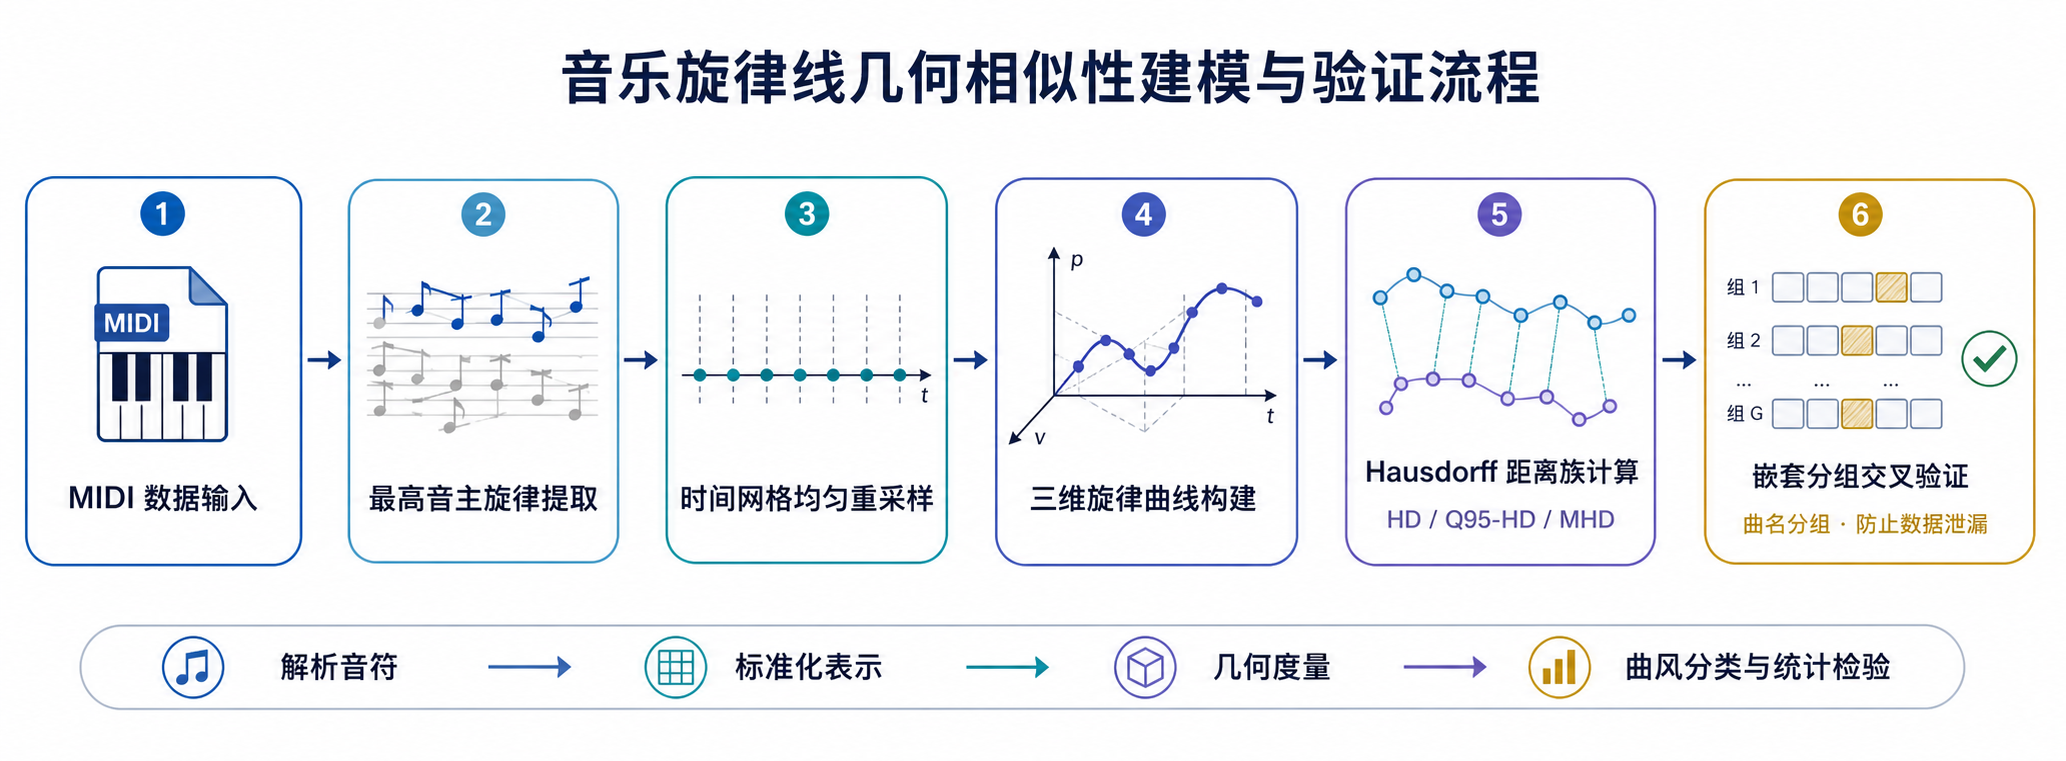
\includegraphics[width=0.98\textwidth]{workflow_gpt_image2.png}
  \caption{本文总体建模与验证流程}
  \label{fig:workflow}
\end{figure}

\subsection{建模难点与本文创新}

优秀的相似性模型不仅要“算得出距离”，还要保证表示合理、验证无泄漏、结论不过度
外推。本文围绕这三点形成表 \ref{tab:innovation} 所示的改进链条。

\begin{table}[!htbp]
  \centering
  \caption{核心难点、解决策略与建模贡献}
  \label{tab:innovation}
  \small
  \begin{tabular}{p{0.21\textwidth}p{0.38\textwidth}p{0.31\textwidth}}
    \toprule
    核心难点 & 解决策略 & 建模贡献\\
    \midrule
    多声部 MIDI 难以直接比较 &
    skyline 主旋律提取、时间相位重采样与相对音高表示 &
    建立统一、可解释的三维旋律曲线\\
    极端音符主导 max-HD &
    引入 Q95-HD 与均值型 MHD，并设置单点扰动实验 &
    将“最坏点差异”改进为稳健的整体形状差异\\
    同曲不同版本造成数据泄漏 &
    跨曲风同名组剔除，规范化曲名分组，嵌套交叉验证 &
    外层结果不含同曲泄漏和测试集调参偏差\\
    显著性不等于实用区分力 &
    同时报告置换检验、配对 AUC、分类精度与 MDS &
    从统计证据和实际效应两方面评价有效性\\
    \bottomrule
  \end{tabular}
\end{table}

\section{模型假设}

\begin{enumerate}[label=\arabic*.]
  \item MIDI 的 note-on 时刻、音高和力度能够近似表示演奏中的旋律事件。
  \item 钢琴编配中同一时刻的最高音通常承载主旋律，因此采用最高音声部
  （skyline）作为主旋律近似。
  \item 同一作品的不同演奏版本不应跨越训练集和测试集；规范化曲名相同的文件
  视为同一分组。
  \item 对曲风而言，绝对调性的重要性低于相对音程结构，因此主模型对音高做
  中位数中心化以获得近似移调不变性。
  \item 五类样本均衡抽取，故随机分类基线为 $1/5=20\%$。
\end{enumerate}

\section{符号说明}

\begin{table}[!htbp]
  \centering
  \caption{主要符号}
  \begin{tabular}{cl}
    \toprule
    符号 & 含义\\
    \midrule
    $M$ & 一首音乐提取出的旋律线点集\\
    $\tau_i,p_i,v_i$ & 第 $i$ 个音符的时间、MIDI 音高和力度\\
    $\bm{x}_i$ & 标准化后的三维旋律点\\
    $h(A,B)$ & 从点集 $A$ 到 $B$ 的有向 Hausdorff 距离\\
    $H(A,B)$ & 双向 max-Hausdorff 距离\\
    $\QHD(A,B)$ & 95\% 分位 Hausdorff 距离\\
    $\MHD(A,B)$ & Modified Hausdorff Distance\\
    $N$ & 旋律曲线的均匀重采样点数\\
    $w_v$ & 音量维权重\\
    $K$ & K-NN 的近邻数\\
    \bottomrule
  \end{tabular}
\end{table}

\section{数据预处理与旋律线构造}

\subsection{数据抽样与防泄漏处理}

ADL Piano MIDI 数据集\cite{adl}包含 18 个目录、共 11076 首钢琴 MIDI。本文选择
Classical、Jazz、Rock、Blues、Electronic 五类。先把文件名转为小写，去除标点、
括号中的版本说明以及明确的 ``take/live/remaster/version'' 后缀，同时保留
``Sinfonia 5'' 一类作品编号，得到规范化曲名。若同一规范化曲名出现在多个曲风
目录，则将其全部排除，共排除 68 个跨曲风标题组；随后以随机种子 2026 打乱
候选曲名组，每组只选取一个可成功解析的版本，每类取 80 首，最终得到 400 首、
400 个独立曲名组。

这一处理比简单取文件夹中按字母排序的前若干首更可靠：它避免了字母顺序偏差，
也防止 ``take 1/take 2''、``live/album version'' 等近重复作品造成测试泄漏。

\subsection{主旋律提取}

本文自行解析标准 MIDI 文件中的变长时间编码、运行状态和 note-on 事件，不依赖
额外 MIDI 库。对每个起始时刻 $\tau$，若同时出现多个音符，保留音高最大的音符：
\begin{equation}
  (p_\tau,v_\tau)
  =\arg\max_{(p,v)\in C_\tau} (p,v),
\end{equation}
其中按音高优先、力度次优作字典序比较；因此最高音并列时保留力度更大的音符。
$C_\tau$ 为时刻 $\tau$ 的同时发声音符集合。少于 32 个主旋律起音的文件被视为
信息不足并跳过。

\subsection{时间均匀重采样}

将相邻旋律点用线段连接。设首末音时刻为 $\tau_{\min},\tau_{\max}$，定义归一化
相位
\begin{equation}
  t_i=\frac{\tau_i-\tau_{\min}}{\tau_{\max}-\tau_{\min}}\in[0,1].
\end{equation}
在 $[0,1]$ 上均匀取 $N$ 个采样点，对音高和力度作分段线性插值。固定基准使用
$N=96$，最终模型在 $N\in\{48,72,96\}$ 中由内层验证选择。本文不采用原有
的三维弧长重采样，因为弧长会被音高和力度量纲主导，使“采样位置”和“距离权重”
相互耦合。图 \ref{fig:curves} 给出五类样本的三维曲线示例。

\begin{figure}[!htbp]
  \centering
  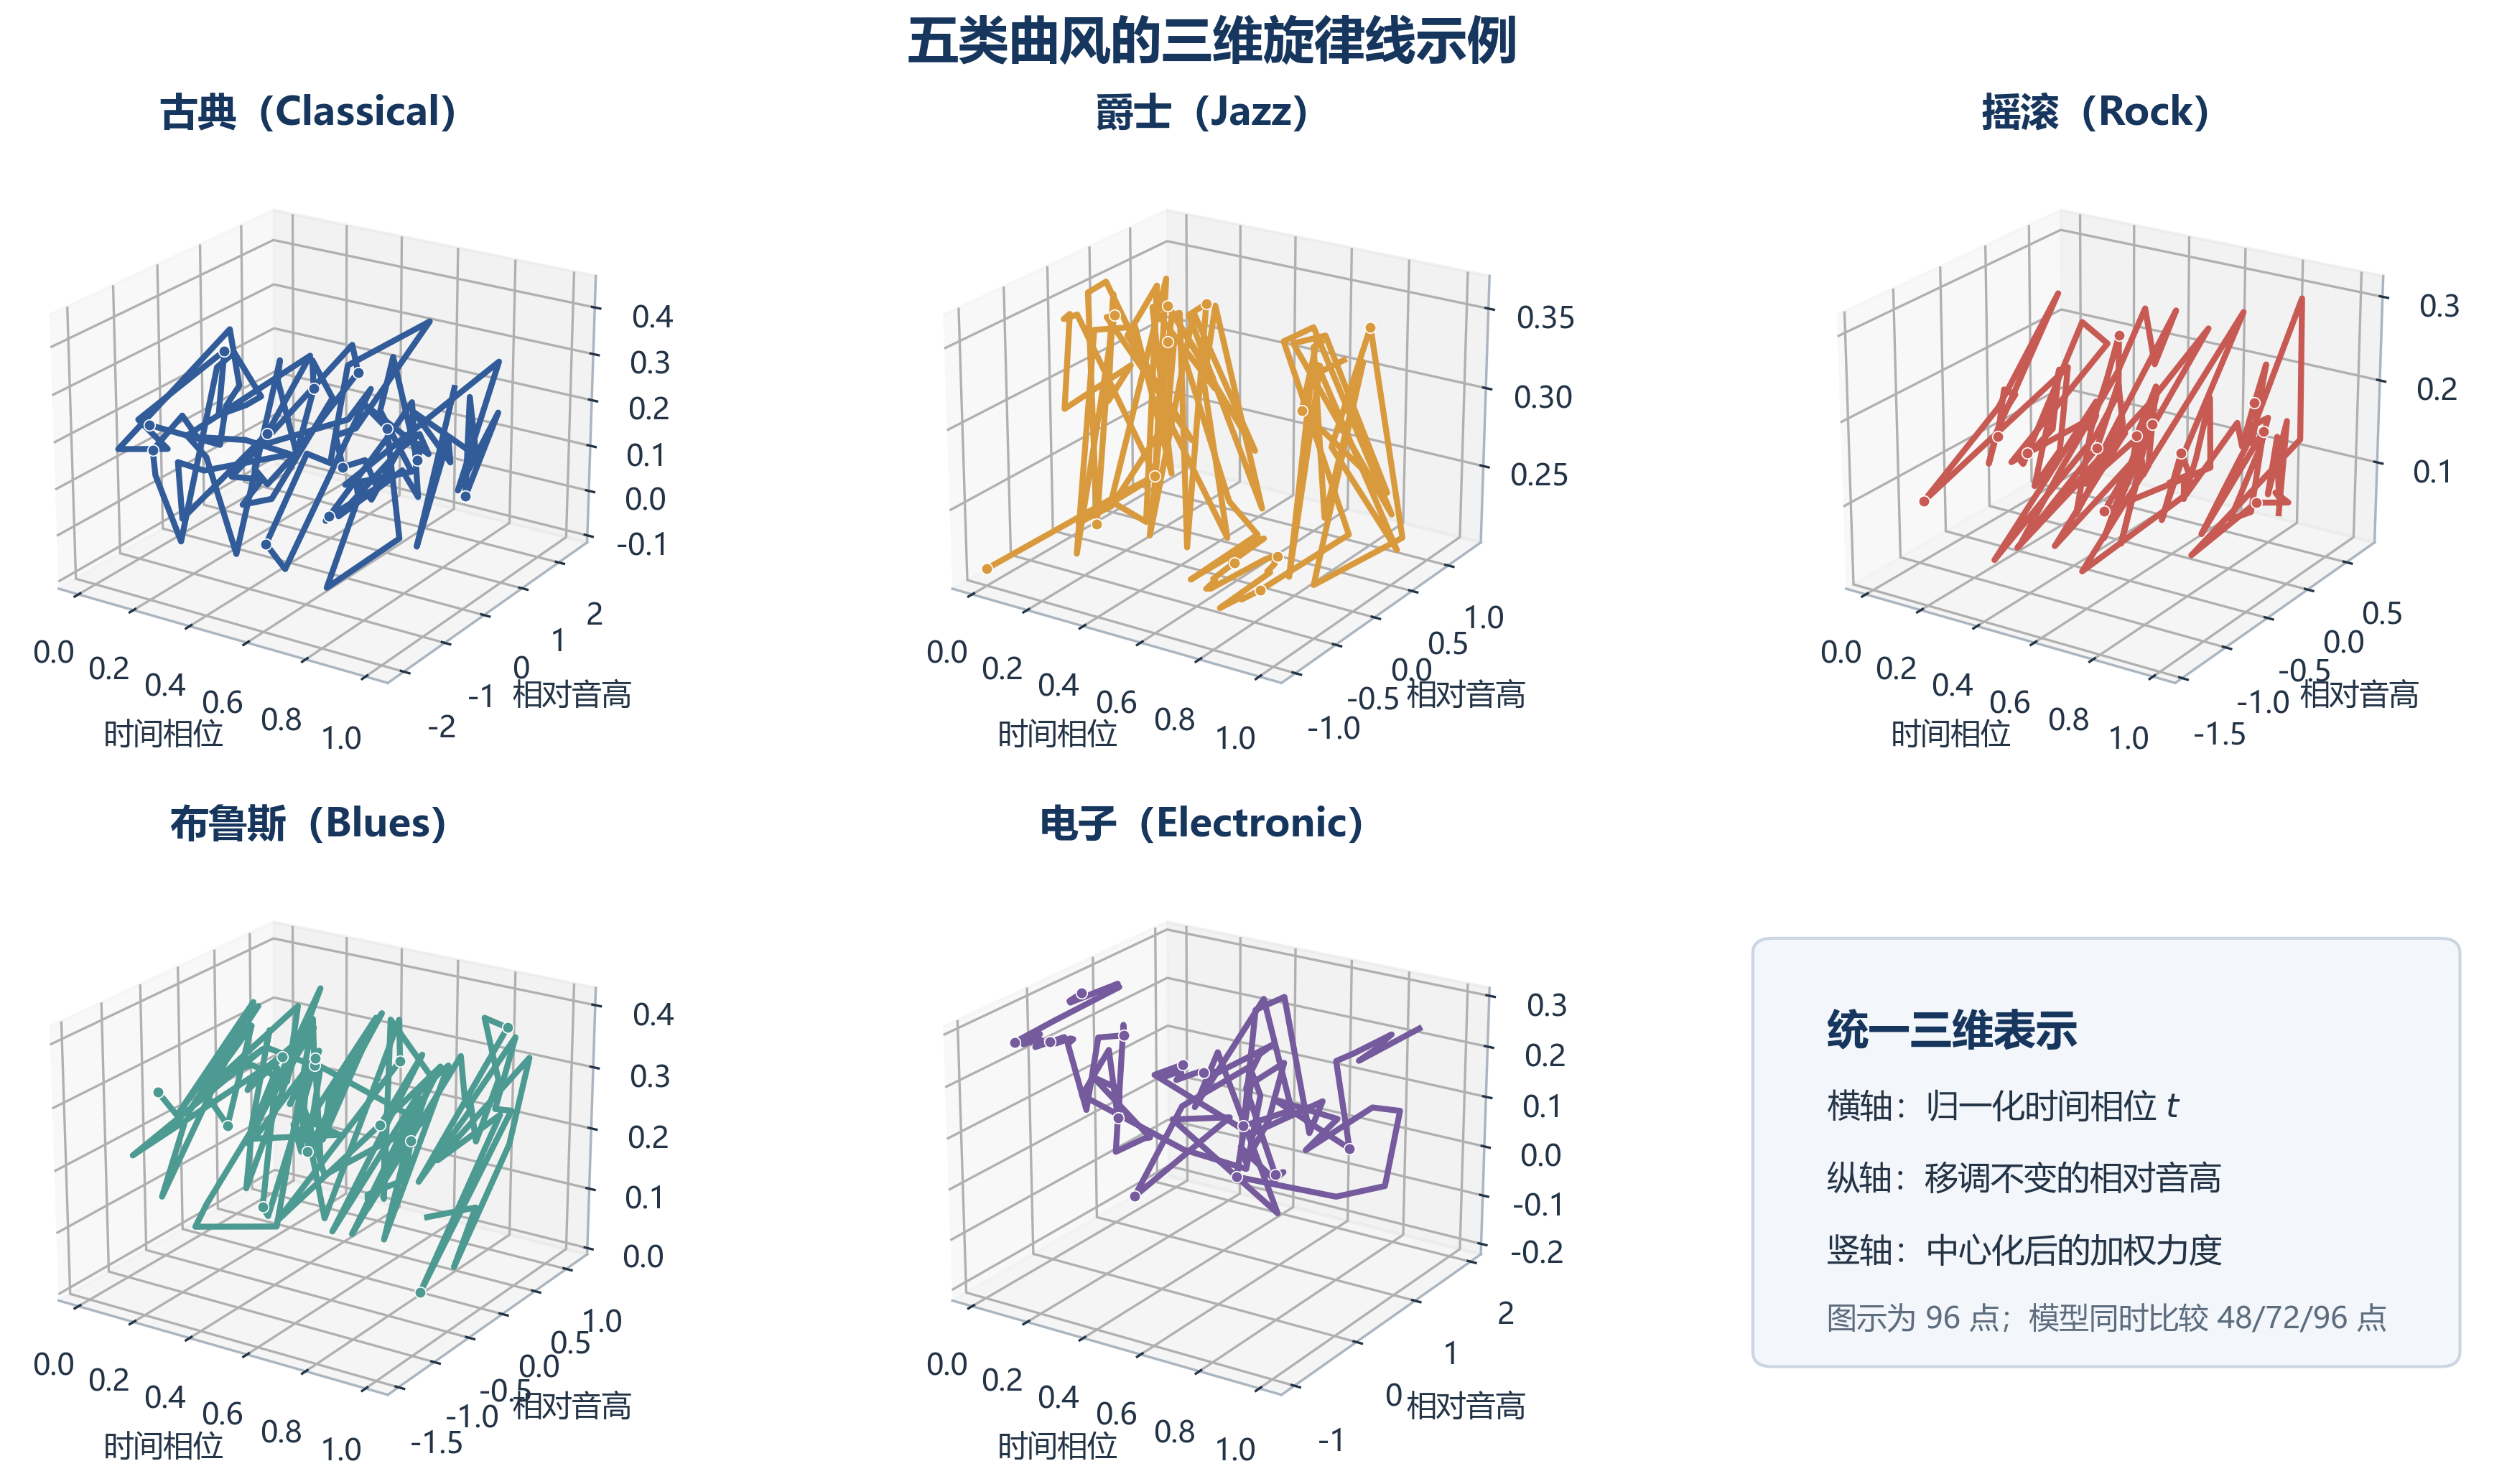
\includegraphics[width=0.98\textwidth]{example_curves_cn.png}
  \caption{五类曲风的标准化三维旋律线示例}
  \label{fig:curves}
\end{figure}

\subsection{相对音高与加权三维表示}

为近似消除移调影响，将音高相对其中位数表示，并按八度缩放；力度以 64 为中心、
32 为尺度。第 $i$ 个三维点写为
\begin{equation}
  \bm{x}_i(w_v)=
  \left(
  t_i,\;
  \frac{p_i-\operatorname{median}(p)}{12},\;
  w_v\frac{v_i-64}{32}
  \right)\in\R^3 .
  \label{eq:representation}
\end{equation}
这样，时间相位 1、一个八度音高差和 $32/w_v$ 个力度单位处于可解释的尺度上。

\section{距离模型的建立}

\subsection{标准 Hausdorff 距离}

对两条旋律线点集\cite{hausdorff} $A=\{\bm a_i\}_{i=1}^{m}$、
$B=\{\bm b_j\}_{j=1}^{n}$，定义有向距离
\begin{equation}
  h(A,B)=\max_{\bm a\in A}\min_{\bm b\in B}
  \|\bm a-\bm b\|_2,
\end{equation}
双向 Hausdorff 距离为
\begin{equation}
  H(A,B)=\max\{h(A,B),h(B,A)\}.
  \label{eq:hd}
\end{equation}
本文用 KD-tree 搜索最近点，使单次有向匹配由朴素的 $O(mn)$ 降为近似
$O(m\log n)$。

\subsection{95\% 分位 Hausdorff}

为减少单个异常音符对最大值的控制，将有向最近距离集合的最大值替换为
95\% 分位数：
\begin{equation}
  \QHD(A,B)=\max\left\{
  Q_{0.95}\!\left(\min_{\bm b\in B}\|\bm a-\bm b\|_2\right),
  Q_{0.95}\!\left(\min_{\bm a\in A}\|\bm b-\bm a\|_2\right)
  \right\}.
\end{equation}

\subsection{Modified Hausdorff Distance}

进一步采用 Dubuisson--Jain 型均值思想\cite{dubuisson}，把最坏点改为整体平均偏差：
\begin{align}
  h_{\mathrm{MHD}}(A,B)
  &=\frac{1}{|A|}\sum_{\bm a\in A}
  \min_{\bm b\in B}\|\bm a-\bm b\|_2,\\
  \MHD(A,B)
  &=\max\{h_{\mathrm{MHD}}(A,B),h_{\mathrm{MHD}}(B,A)\}.
  \label{eq:mhd}
\end{align}
外层保留双向最大值，以防止稠密短曲线被稀疏长曲线单向“覆盖”。

\subsection{嵌套多参数 MHD}

固定离散密度和音量权重可能不适合所有训练划分。本文令
\begin{equation}
  N\in\{48,72,96\},\qquad
  w_v\in\{0,0.1,0.25,0.5\},\qquad
  K\in\{1,3,5,7,9\},
\end{equation}
在每个外层训练集内部，以 3 个随机种子分别进行三折分组交叉验证，联合选择
\begin{equation}
  (N^\ast,w_v^\ast,K^\ast)
  =\arg\max_{N,w_v,K}\overline{\operatorname{BAcc}}_{\mathrm{inner}}(N,w_v,K).
\end{equation}
随后仅在该外层测试折上评估一次，得到无测试集调参偏差的性能估计。

\subsection{对照模型}

本文设置两类对照：
\begin{enumerate}[label=(\arabic*)]
  \item \textbf{DTW 相对音高距离：}保留时序顺序，以 Sakoe--Chiba 窗口\cite{dtw}对齐
  相对音高序列；
  \item \textbf{随机森林描述符模型：}采用随机森林\cite{rf}并提取 40 个可解释特征，包括时长、音符
  密度、音域、音程、力度、相邻起音间隔、切分比例、12 维音级直方图等。该模型
  不属于纯几何距离，而作为融合全局统计信息后的能力对照。
\end{enumerate}

\section{模型求解与评价方案}

\subsection{嵌套分组五折交叉验证}

外层采用 Stratified Group 5-Fold：尽量保持各曲风比例，同时保证相同规范化
曲名只出现在一个折中。距离 K-NN 的 $N,w_v,K$ 在外层训练数据上通过
3 组内层三折的平均平衡准确率确定。
所有结果报告外层 5 个测试折的均值和样本标准差。评价指标包括准确率、平衡
准确率、宏平均 F1 和归一化混淆矩阵。

\subsection{距离分布检验}

将 400 首曲目的所有两两距离分为同曲风组与异曲风组。由于同一曲目参与多个
配对，普通独立样本检验会夸大显著性，因此本文采用 1999 次组级标签置换检验：
以规范化曲名组为单位随机打乱曲风标签，重复计算“异类均值减同类均值”，并以
\begin{equation}
  p=\frac{1+\#\{\Delta_{\mathrm{perm}}\geq\Delta_{\mathrm{obs}}\}}{1999+1}
\end{equation}
估计显著性。同时报告配对 AUC，衡量随机抽取一对同类和一对异类时，前者距离
更小的概率。

\section{模型检验与实验结果}

\begin{figure}[!htbp]
  \centering
  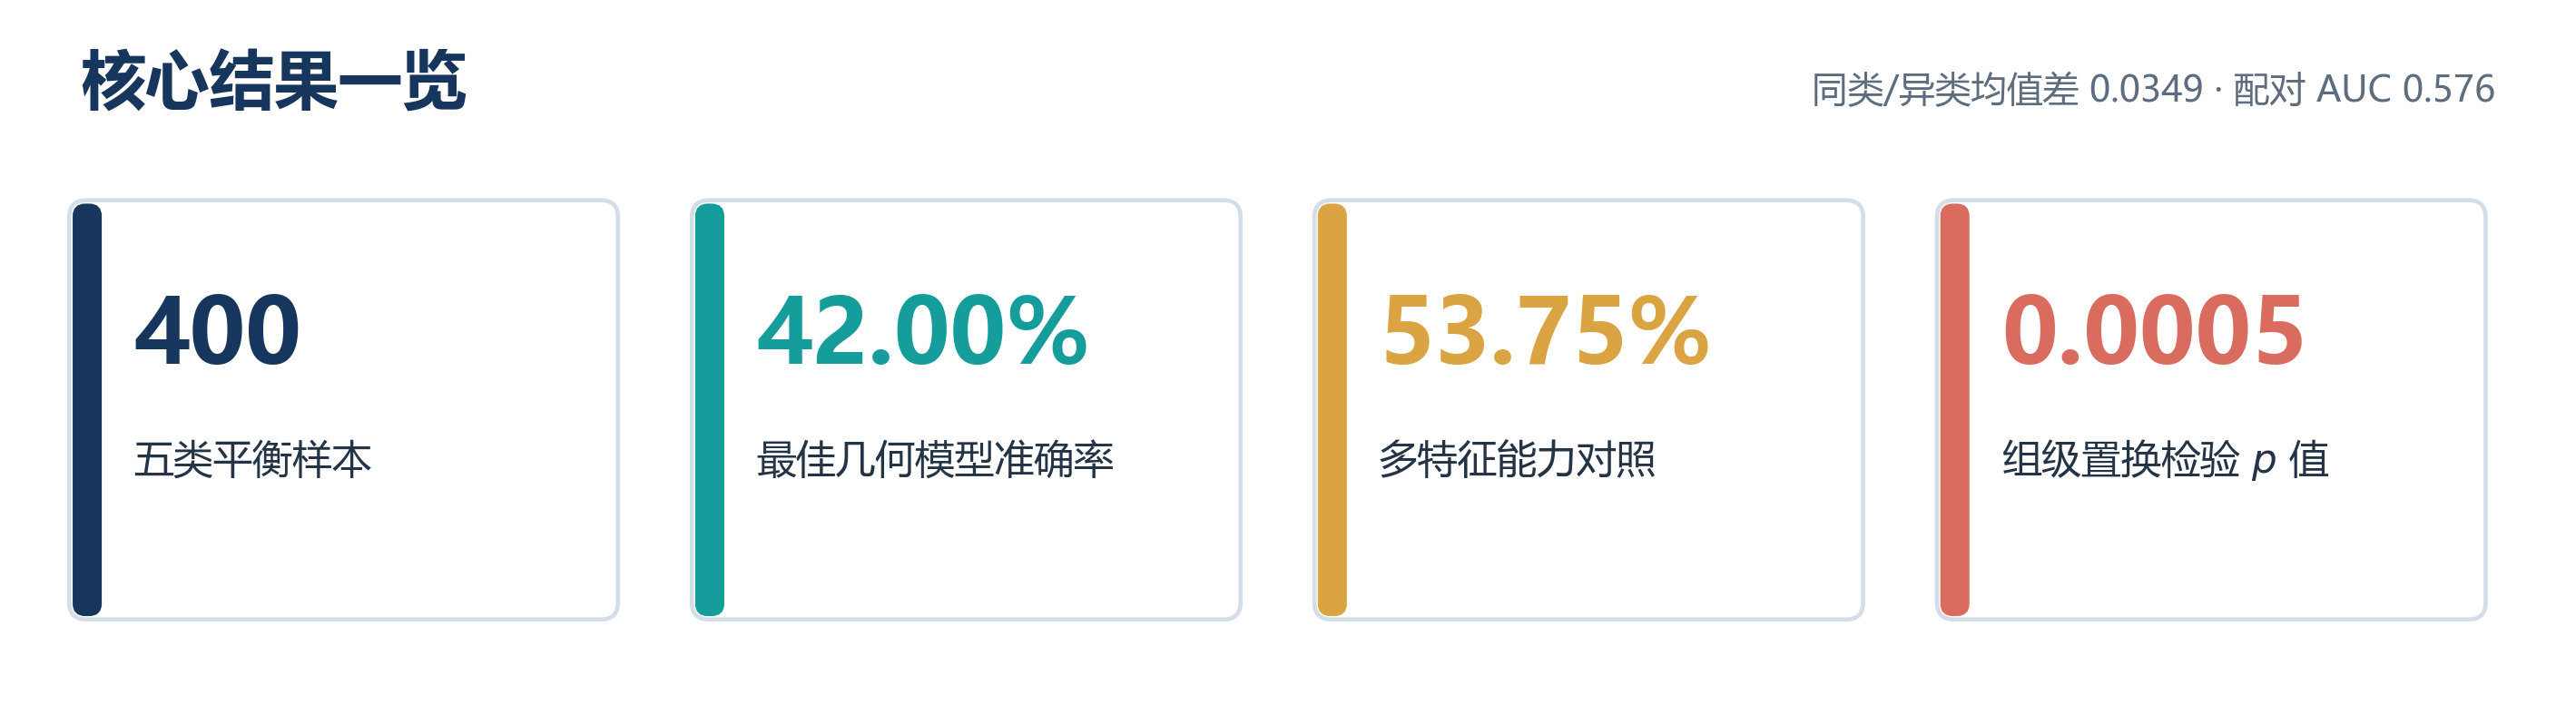
\includegraphics[width=0.98\textwidth]{results_dashboard_cn.png}
  \caption{实验规模与核心结果概览}
  \label{fig:dashboard}
\end{figure}

\subsection{离群点稳健性}

在合成曲线上只扰动一个采样点。图 \ref{fig:synthetic} 显示 max-Hausdorff
随异常幅度迅速增大；95\% 分位距离几乎不受单点影响；MHD 仅缓慢增加。这说明
原始最大值确实容易被单个装饰音或解析误差主导。

\begin{figure}[!htbp]
  \centering
  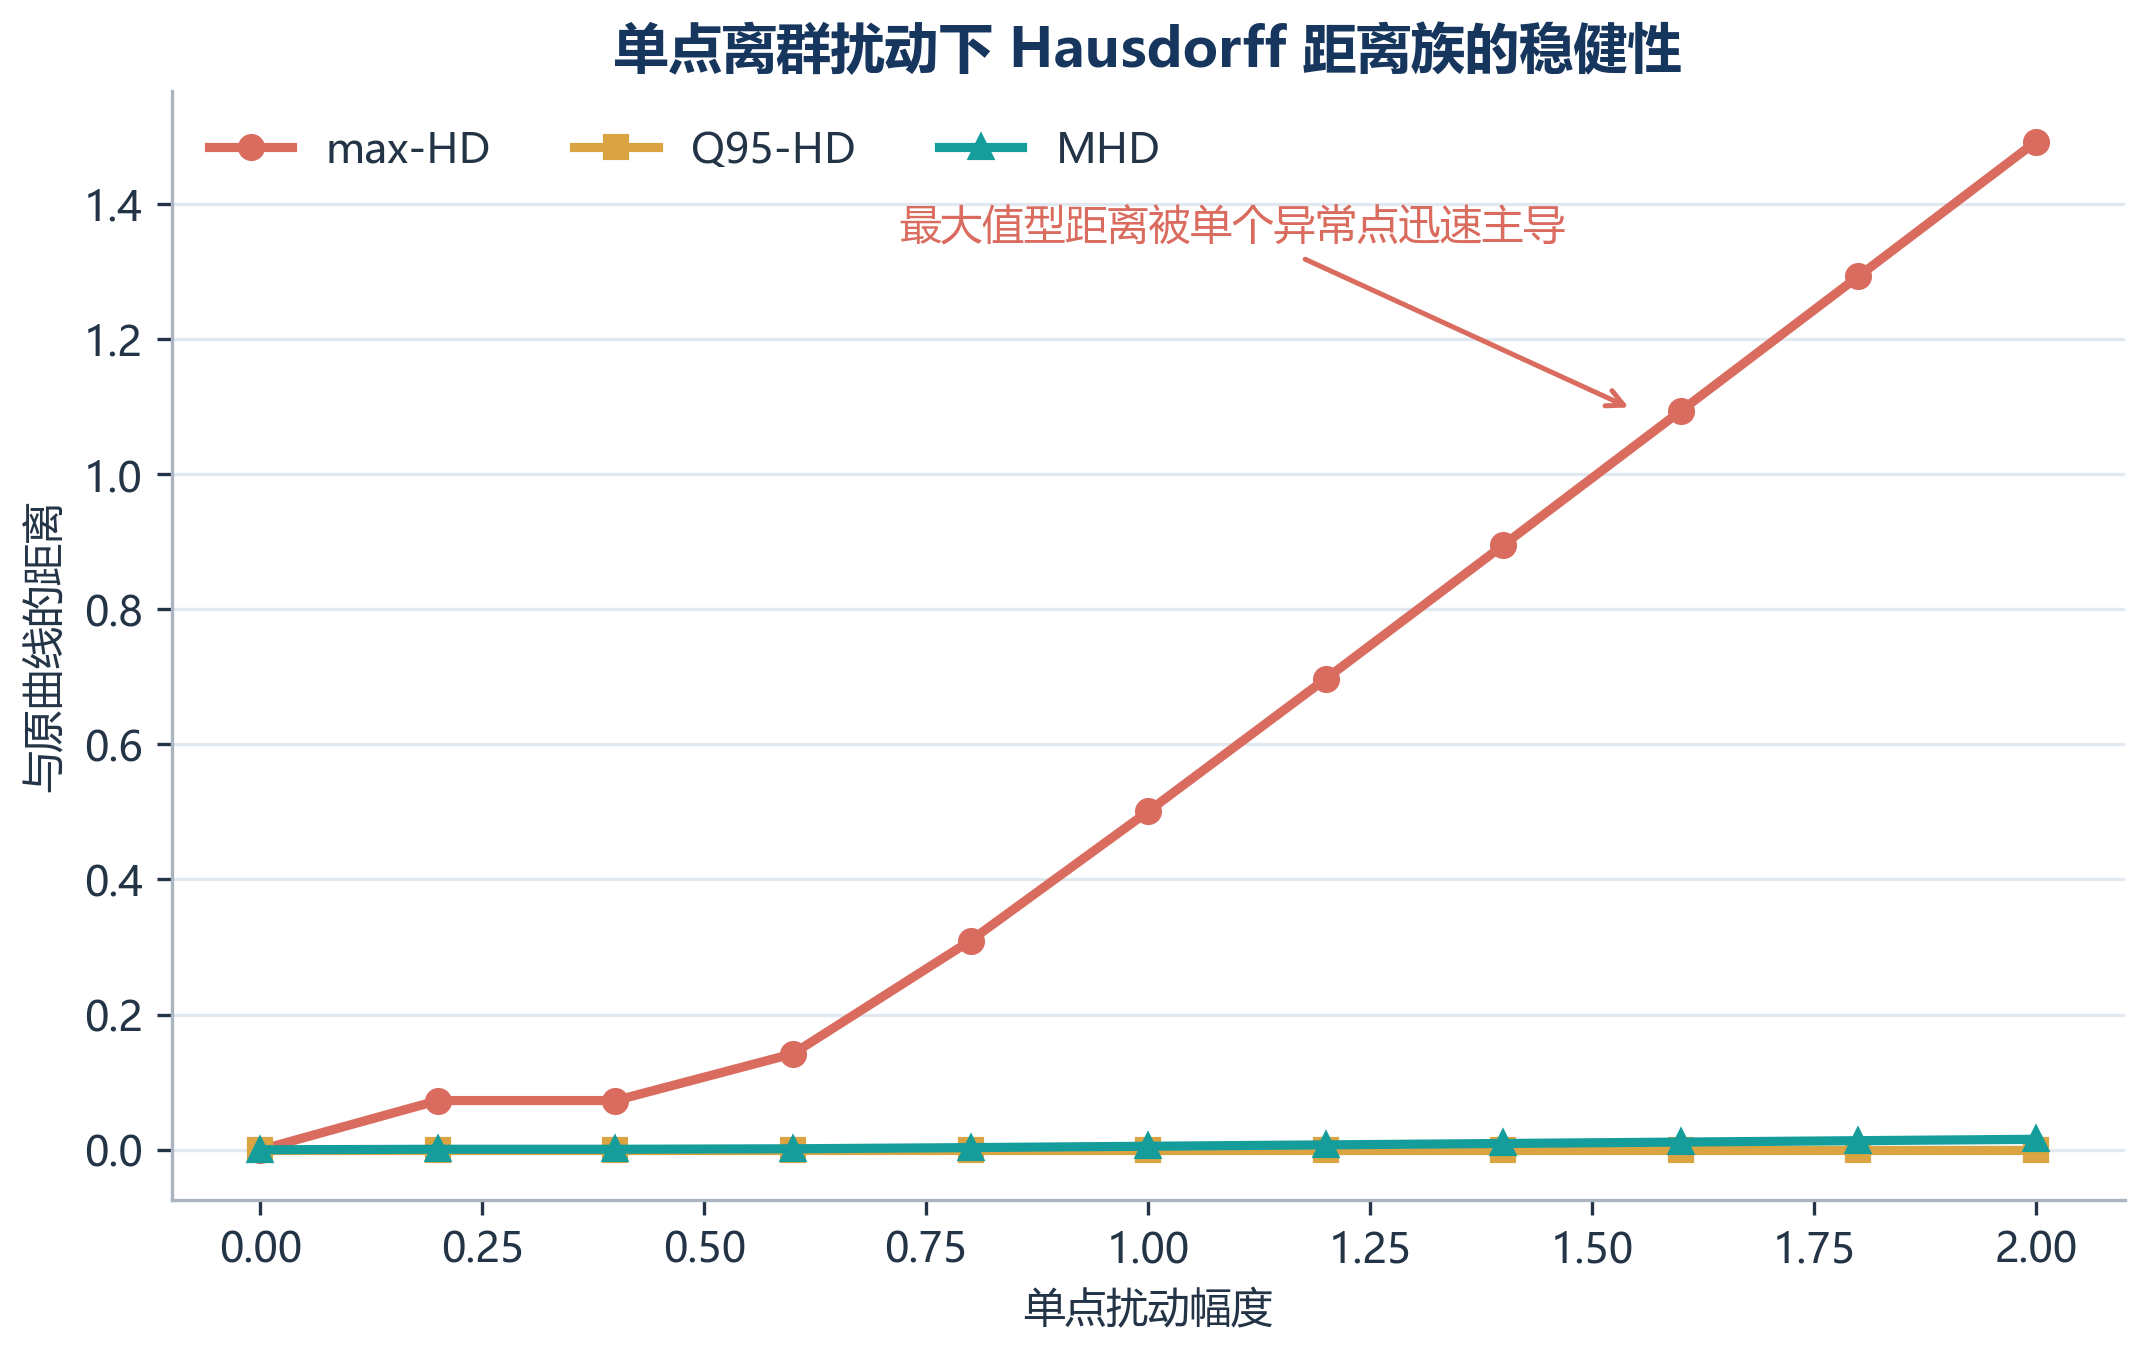
\includegraphics[width=0.82\textwidth]{synthetic_robustness_cn.png}
  \caption{单点离群扰动下三种 Hausdorff 族距离的响应}
  \label{fig:synthetic}
\end{figure}

\subsection{同类与异类距离分布}

固定 $N=96,w_v=0.25$ 时，同类 MHD 均值为 0.3192、中位数为 0.2744；异类均值为
0.3541、中位数为 0.3173，均值差为 0.0349。组级置换检验 $p=0.0005$，拒绝“曲风
标签与距离结构无关”的原假设。配对 AUC 为 0.5759，虽高于 0.5，但仍说明两类
分布高度重叠。

\begin{figure}[!htbp]
  \centering
  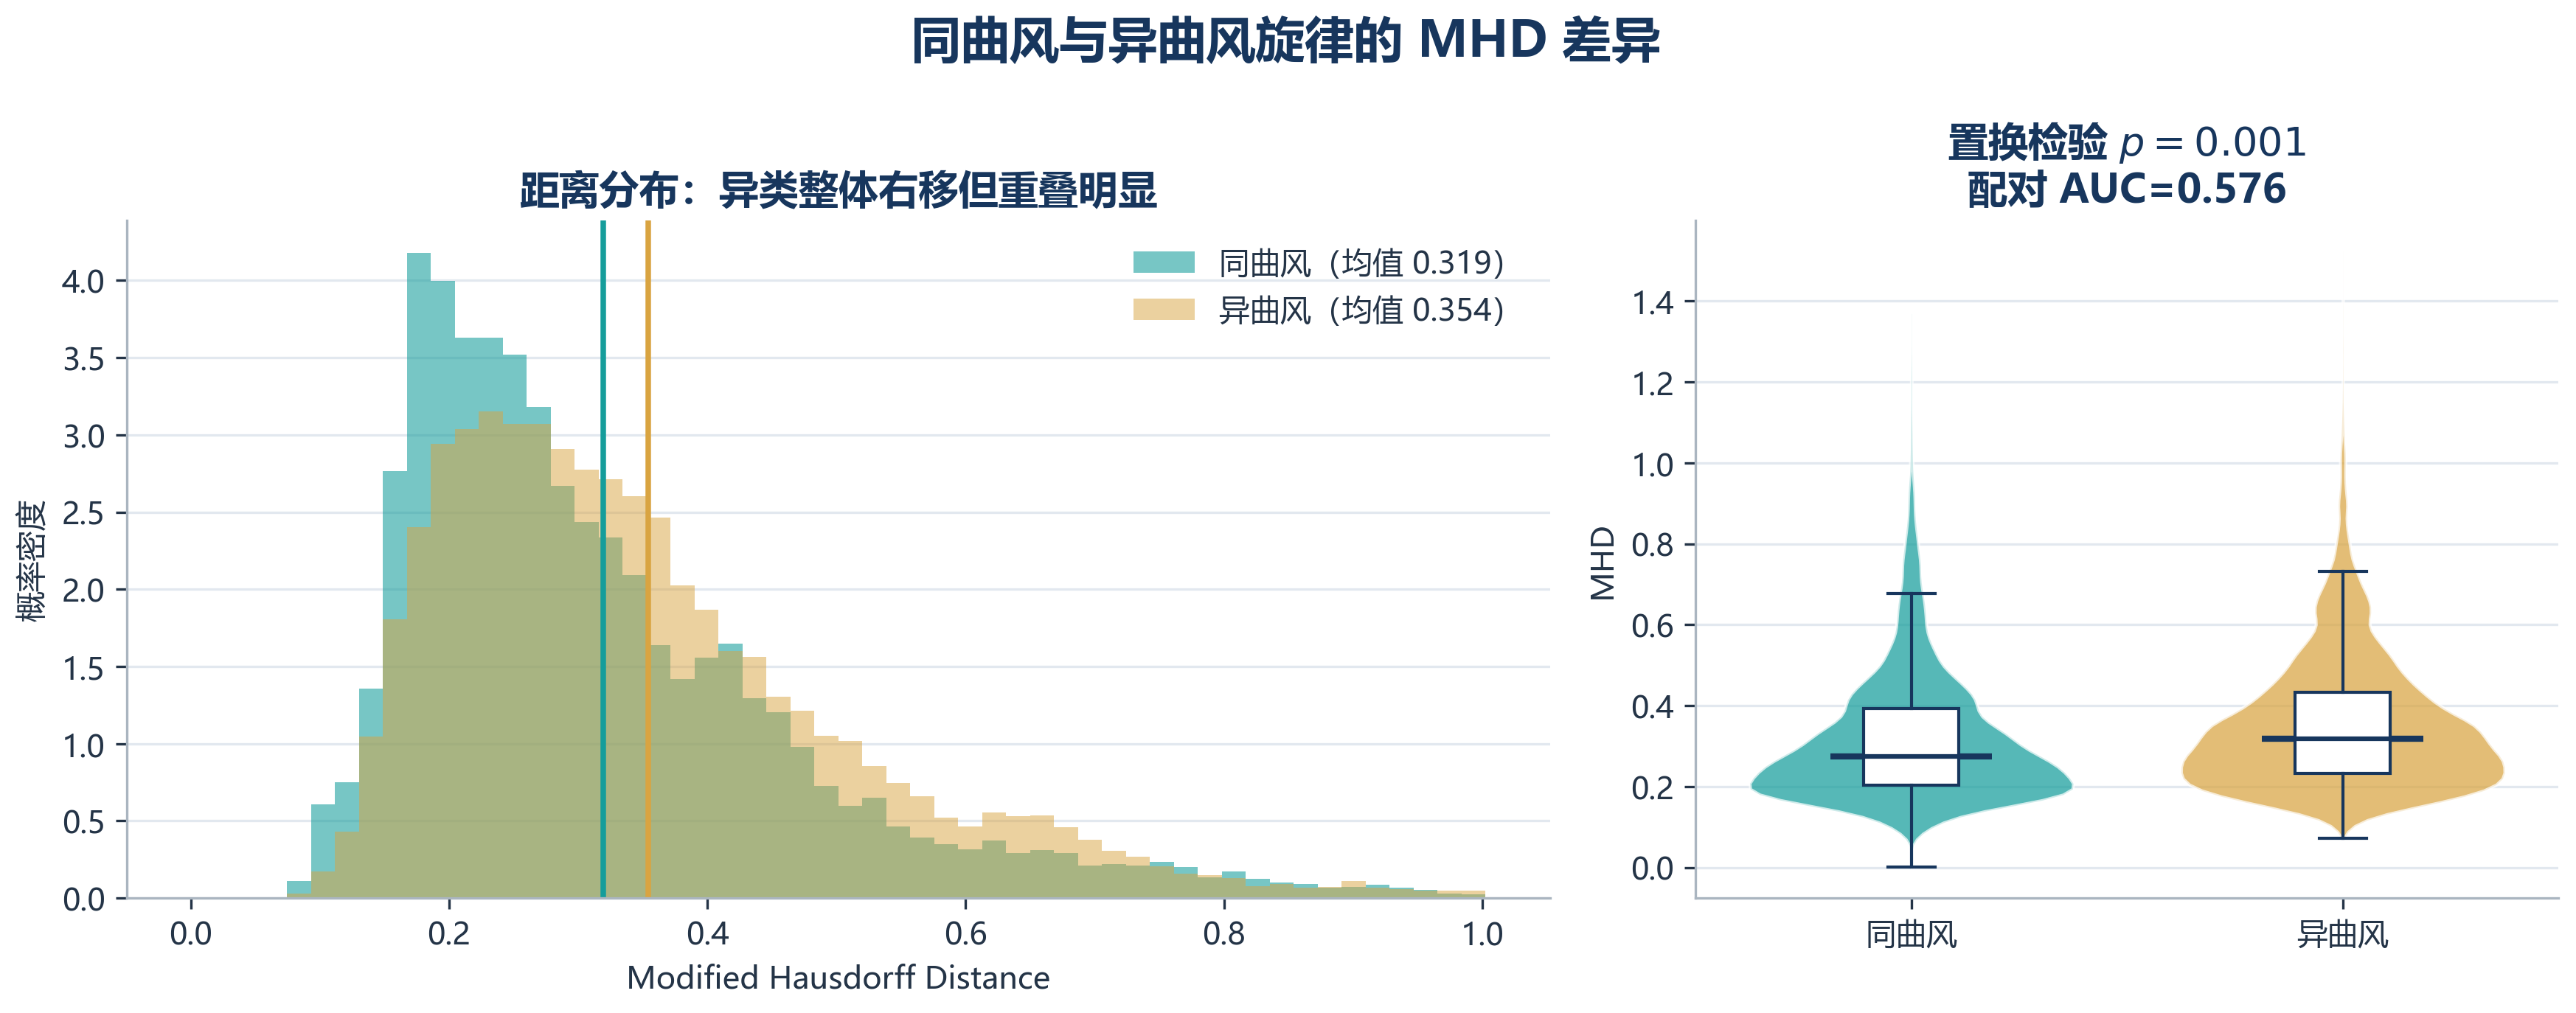
\includegraphics[width=0.98\textwidth]{distance_distribution_cn.png}
  \caption{同曲风与异曲风的 MHD 分布}
  \label{fig:distribution}
\end{figure}

曲风平均距离矩阵见图 \ref{fig:heatmap}。Jazz 与 Blues 的类内均值最低，
分别为 0.267 和 0.269；Electronic 类内均值最高（0.371），表明其内部旋律
形态最分散。Classical--Jazz 的平均距离最大（0.407），而 Rock--Blues
较近（0.316），与后续混淆关系基本一致。

\begin{figure}[!htbp]
  \centering
  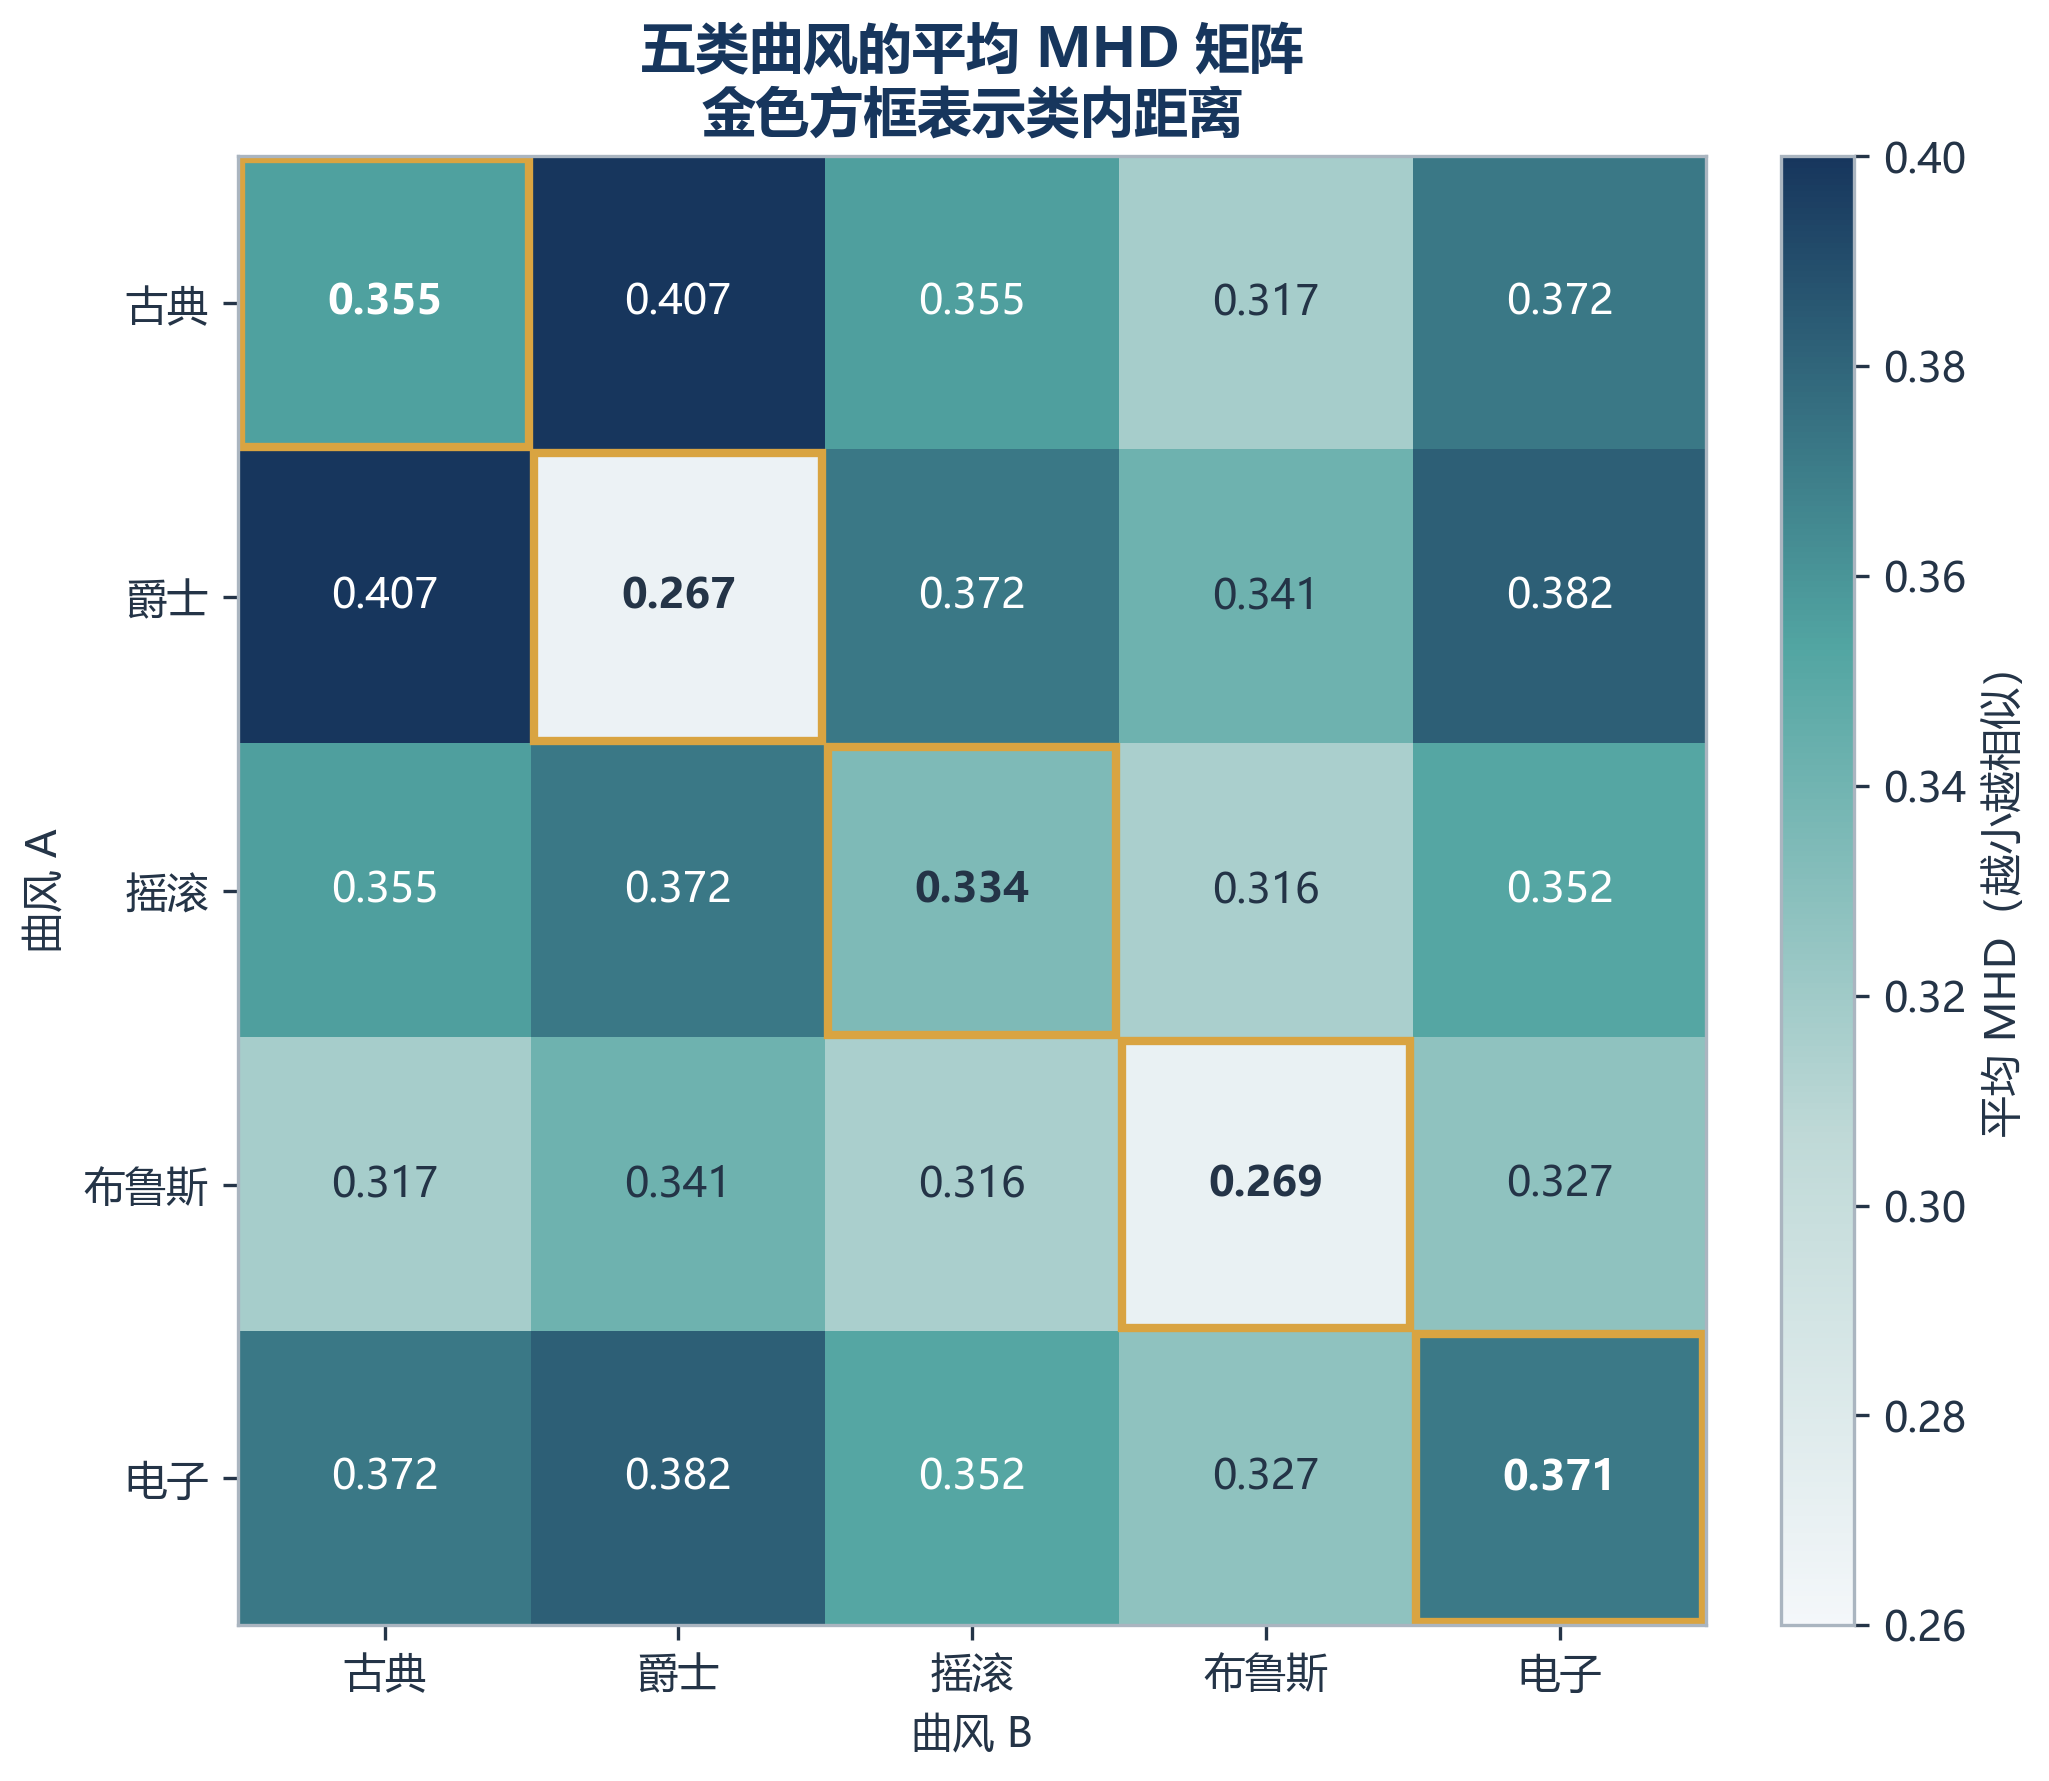
\includegraphics[width=0.62\textwidth]{genre_distance_heatmap_cn.png}
  \caption{五类曲风的平均 MHD 矩阵}
  \label{fig:heatmap}
\end{figure}

\subsection{分类性能比较}

\begin{table}[!htbp]
  \centering
  \begin{threeparttable}
  \caption{不同距离与分类模型的分组五折结果}
  \label{tab:model}
  \small
  \setlength{\tabcolsep}{4.5pt}
  \begin{tabular}{lccc}
    \toprule
    方法 & 准确率（均值$\pm$标准差） & 总体 Macro-F1 & 说明\\
    \midrule
    HD，逐曲 Min--Max & $33.25\%\pm2.88\%$ & 0.306 & 原始基线\\
    HD，相对音高 TP & $32.75\%\pm5.03\%$ & 0.327 & 不使用音量\\
    HD，相对音高 TPV & $32.00\%\pm6.94\%$ & 0.316 & $w_v=0.25$\\
    95\% 分位 HD & $33.75\%\pm3.85\%$ & 0.326 & 抑制极端点\\
    MHD & $38.00\%\pm5.77\%$ & 0.370 & 整体最近距离均值\\
    DTW，相对音高 & $28.50\%\pm2.71\%$ & 0.291 & 时序对照\\
    \rowcolor{papergold!16}
    \textbf{多参数 MHD（嵌套）} & $\bm{42.00\%\pm6.16\%}$ & \textbf{0.410} & 内层选 $N,w_v,K$\\
    \rowcolor{paperblue!9}
    随机森林描述符 & $53.75\%\pm7.50\%$ & 0.541 & 多特征能力对照\\
    \midrule
    随机猜测 & 20.00\% & 0.200 & 五类均衡\\
    \bottomrule
  \end{tabular}
  \begin{tablenotes}
    \small
    \item 注：准确率标准差为五个外层测试折的样本标准差；总体 Macro-F1 由
    400 个外层折外预测合并计算。
  \end{tablenotes}
  \end{threeparttable}
\end{table}

从表 \ref{tab:model} 可得：
\begin{enumerate}[label=\arabic*.]
  \item 所有 Hausdorff 族模型均明显高于 20\% 随机基线，说明三维旋律几何
  结构含有可利用的曲风信息。
  \item MHD 比固定权重三维 max-Hausdorff 提升 6.0 个百分点，支持
  “整体形状比最坏点更适合曲风区分”的判断。
  \item 嵌套多参数 MHD 达到 42.00\%，比固定 MHD 提高 4.00 个百分点。
  五个外层折中有四折选择 $w_v=0.5$；采样点数依次选择 96、96、48、48、72，
  说明力度维度有信息，但不存在对所有划分都最优的单一离散密度。
  \item 本实验中的 DTW 仅使用相对音高，未利用节奏和力度，因此低于三维 MHD；
  这并不意味着所有 DTW 变体都弱于 Hausdorff。
  \item 随机森林仍比最佳几何模型高 11.75 个百分点，说明曲风差异还依赖曲长、
  节奏密度、音级分布和动态范围等全局统计，单一曲线距离不能完整表达。
\end{enumerate}

\begin{figure}[!htbp]
  \centering
  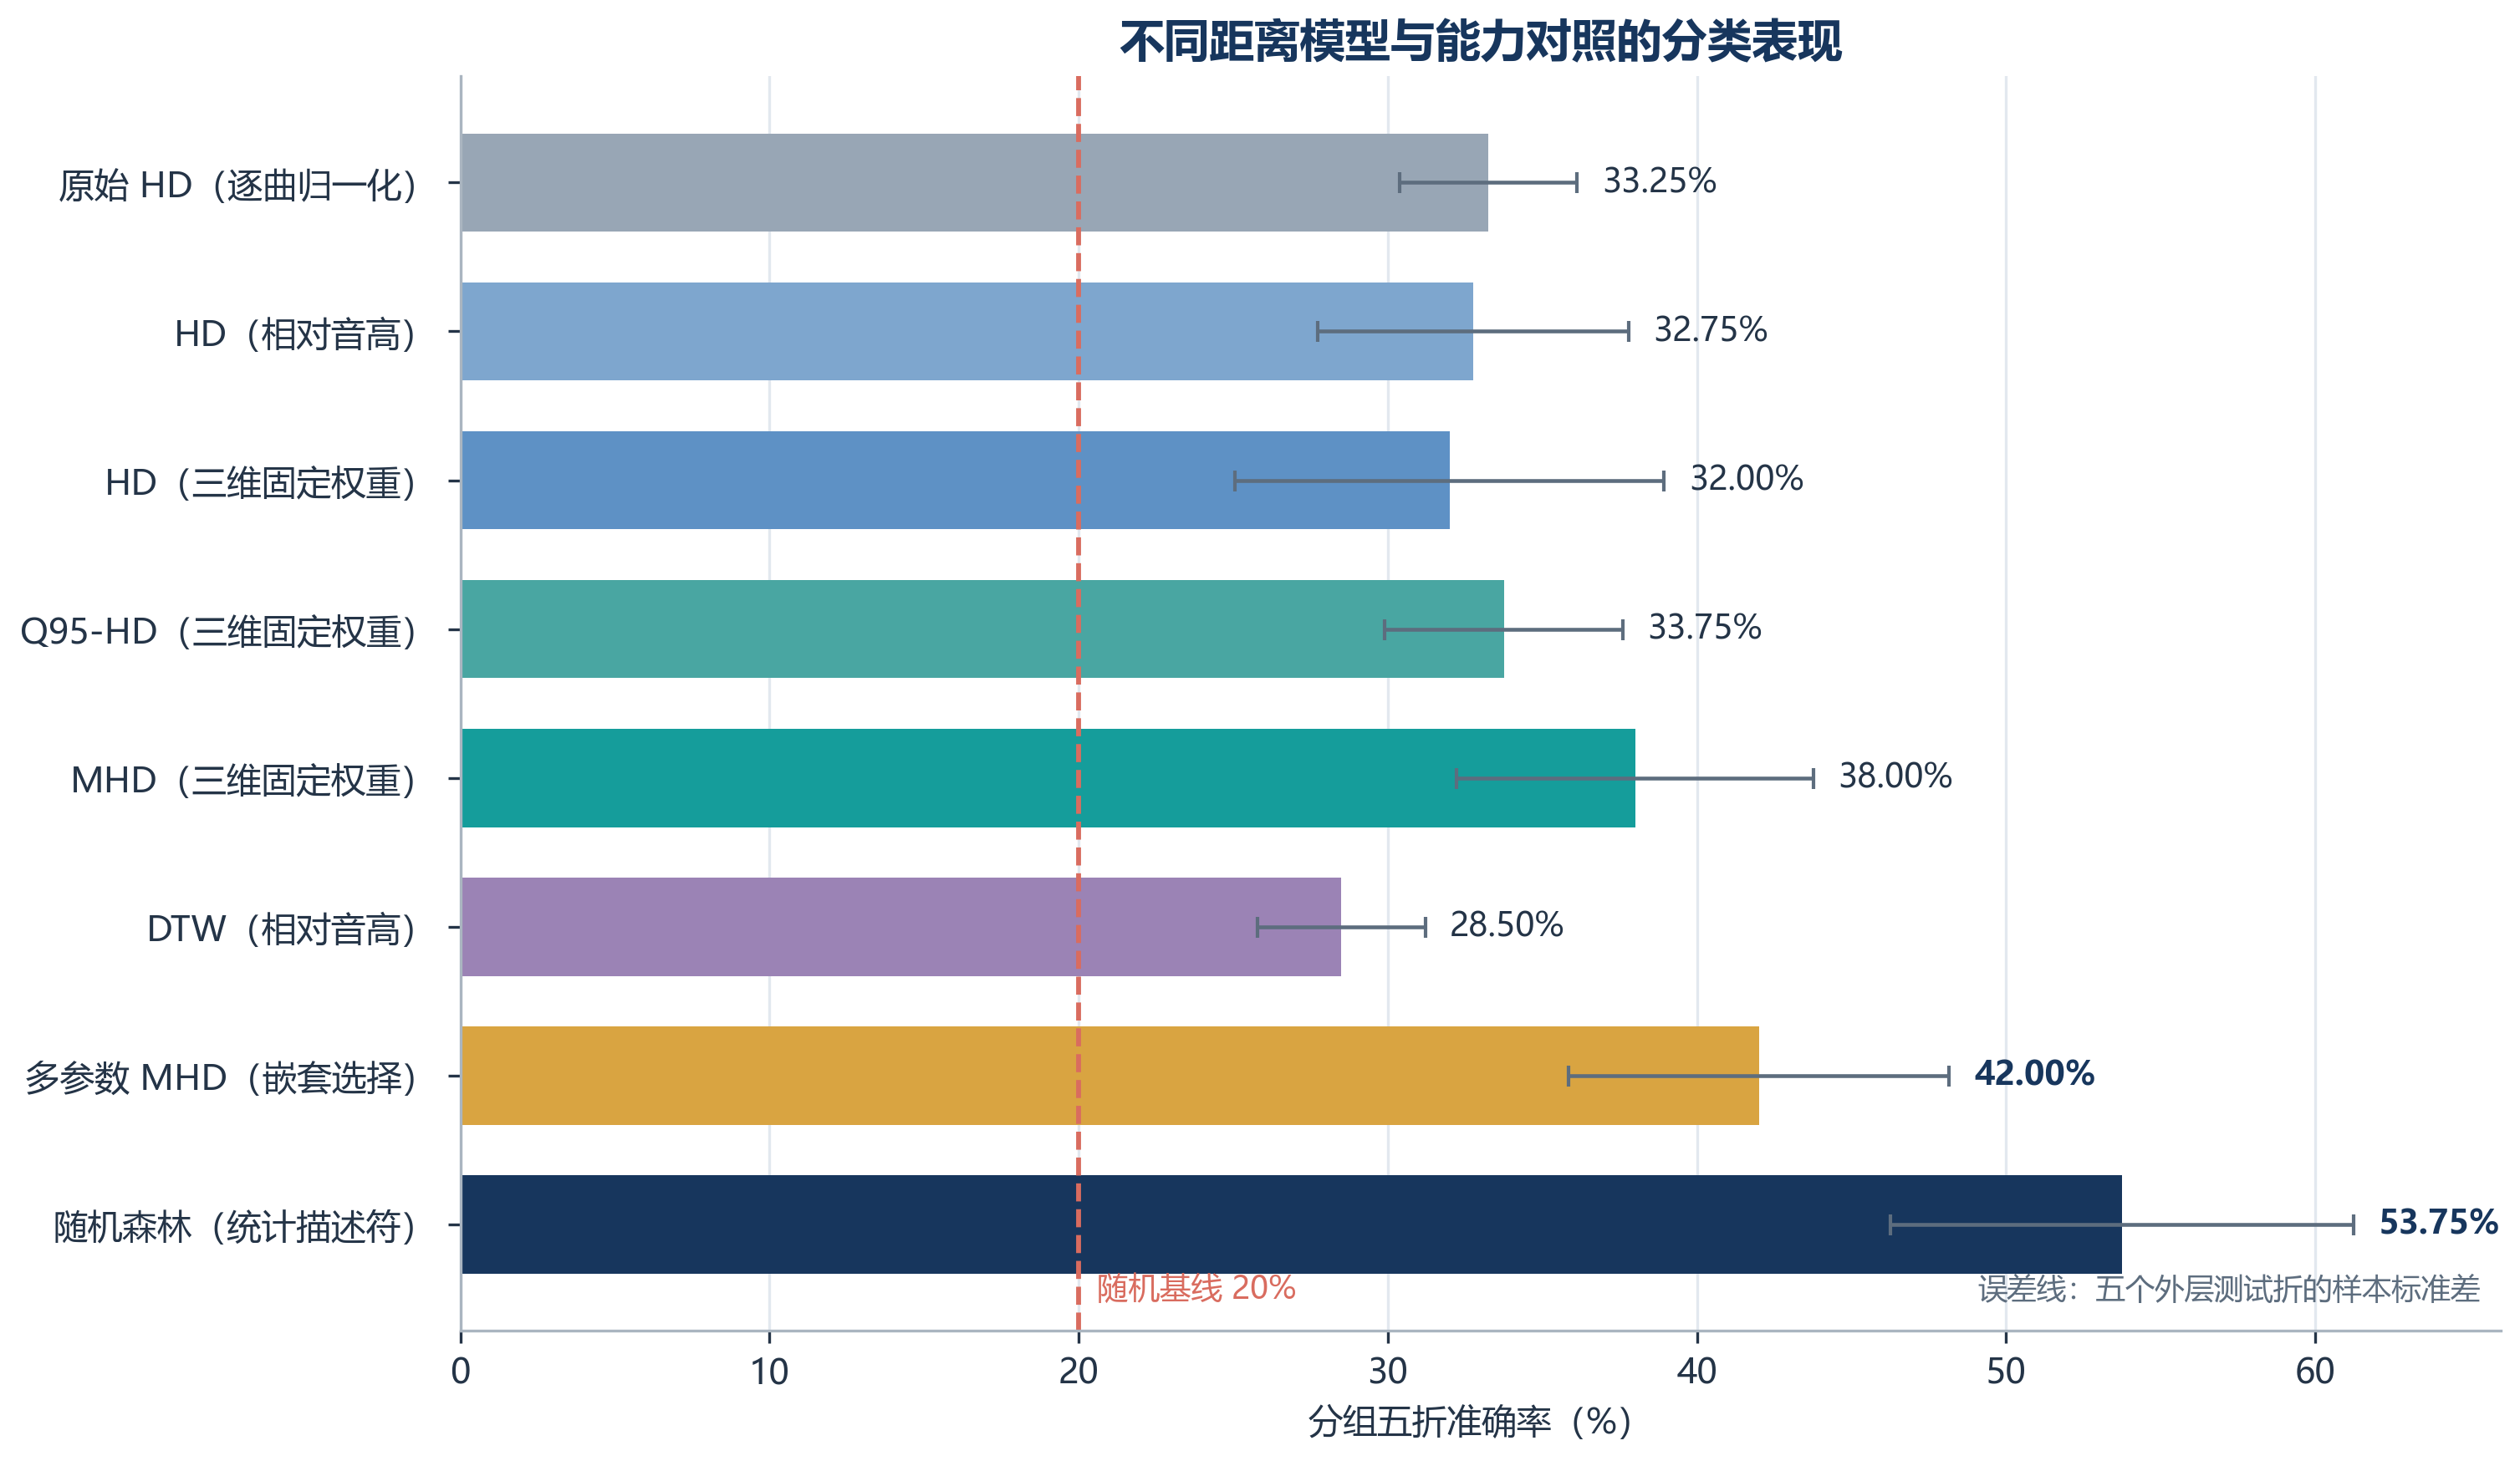
\includegraphics[width=0.98\textwidth]{model_comparison_cn.png}
  \caption{各模型分组五折准确率比较}
  \label{fig:modelcompare}
\end{figure}

\subsection{混淆结构与可视化}

最佳多参数 MHD 的折外混淆矩阵见图 \ref{fig:cmhd}。Classical 与 Jazz 的召回率
分别为 65.0\% 和 58.8\%，而 Rock、Blues、Electronic 分别为 27.5\%、33.8\%
和 25.0\%。Rock 易被判为 Classical 或 Blues，Electronic 易被判为 Rock 或
Blues，说明“几何外形相近”并不等同于“曲风相同”。

\begin{figure}[!htbp]
  \centering
  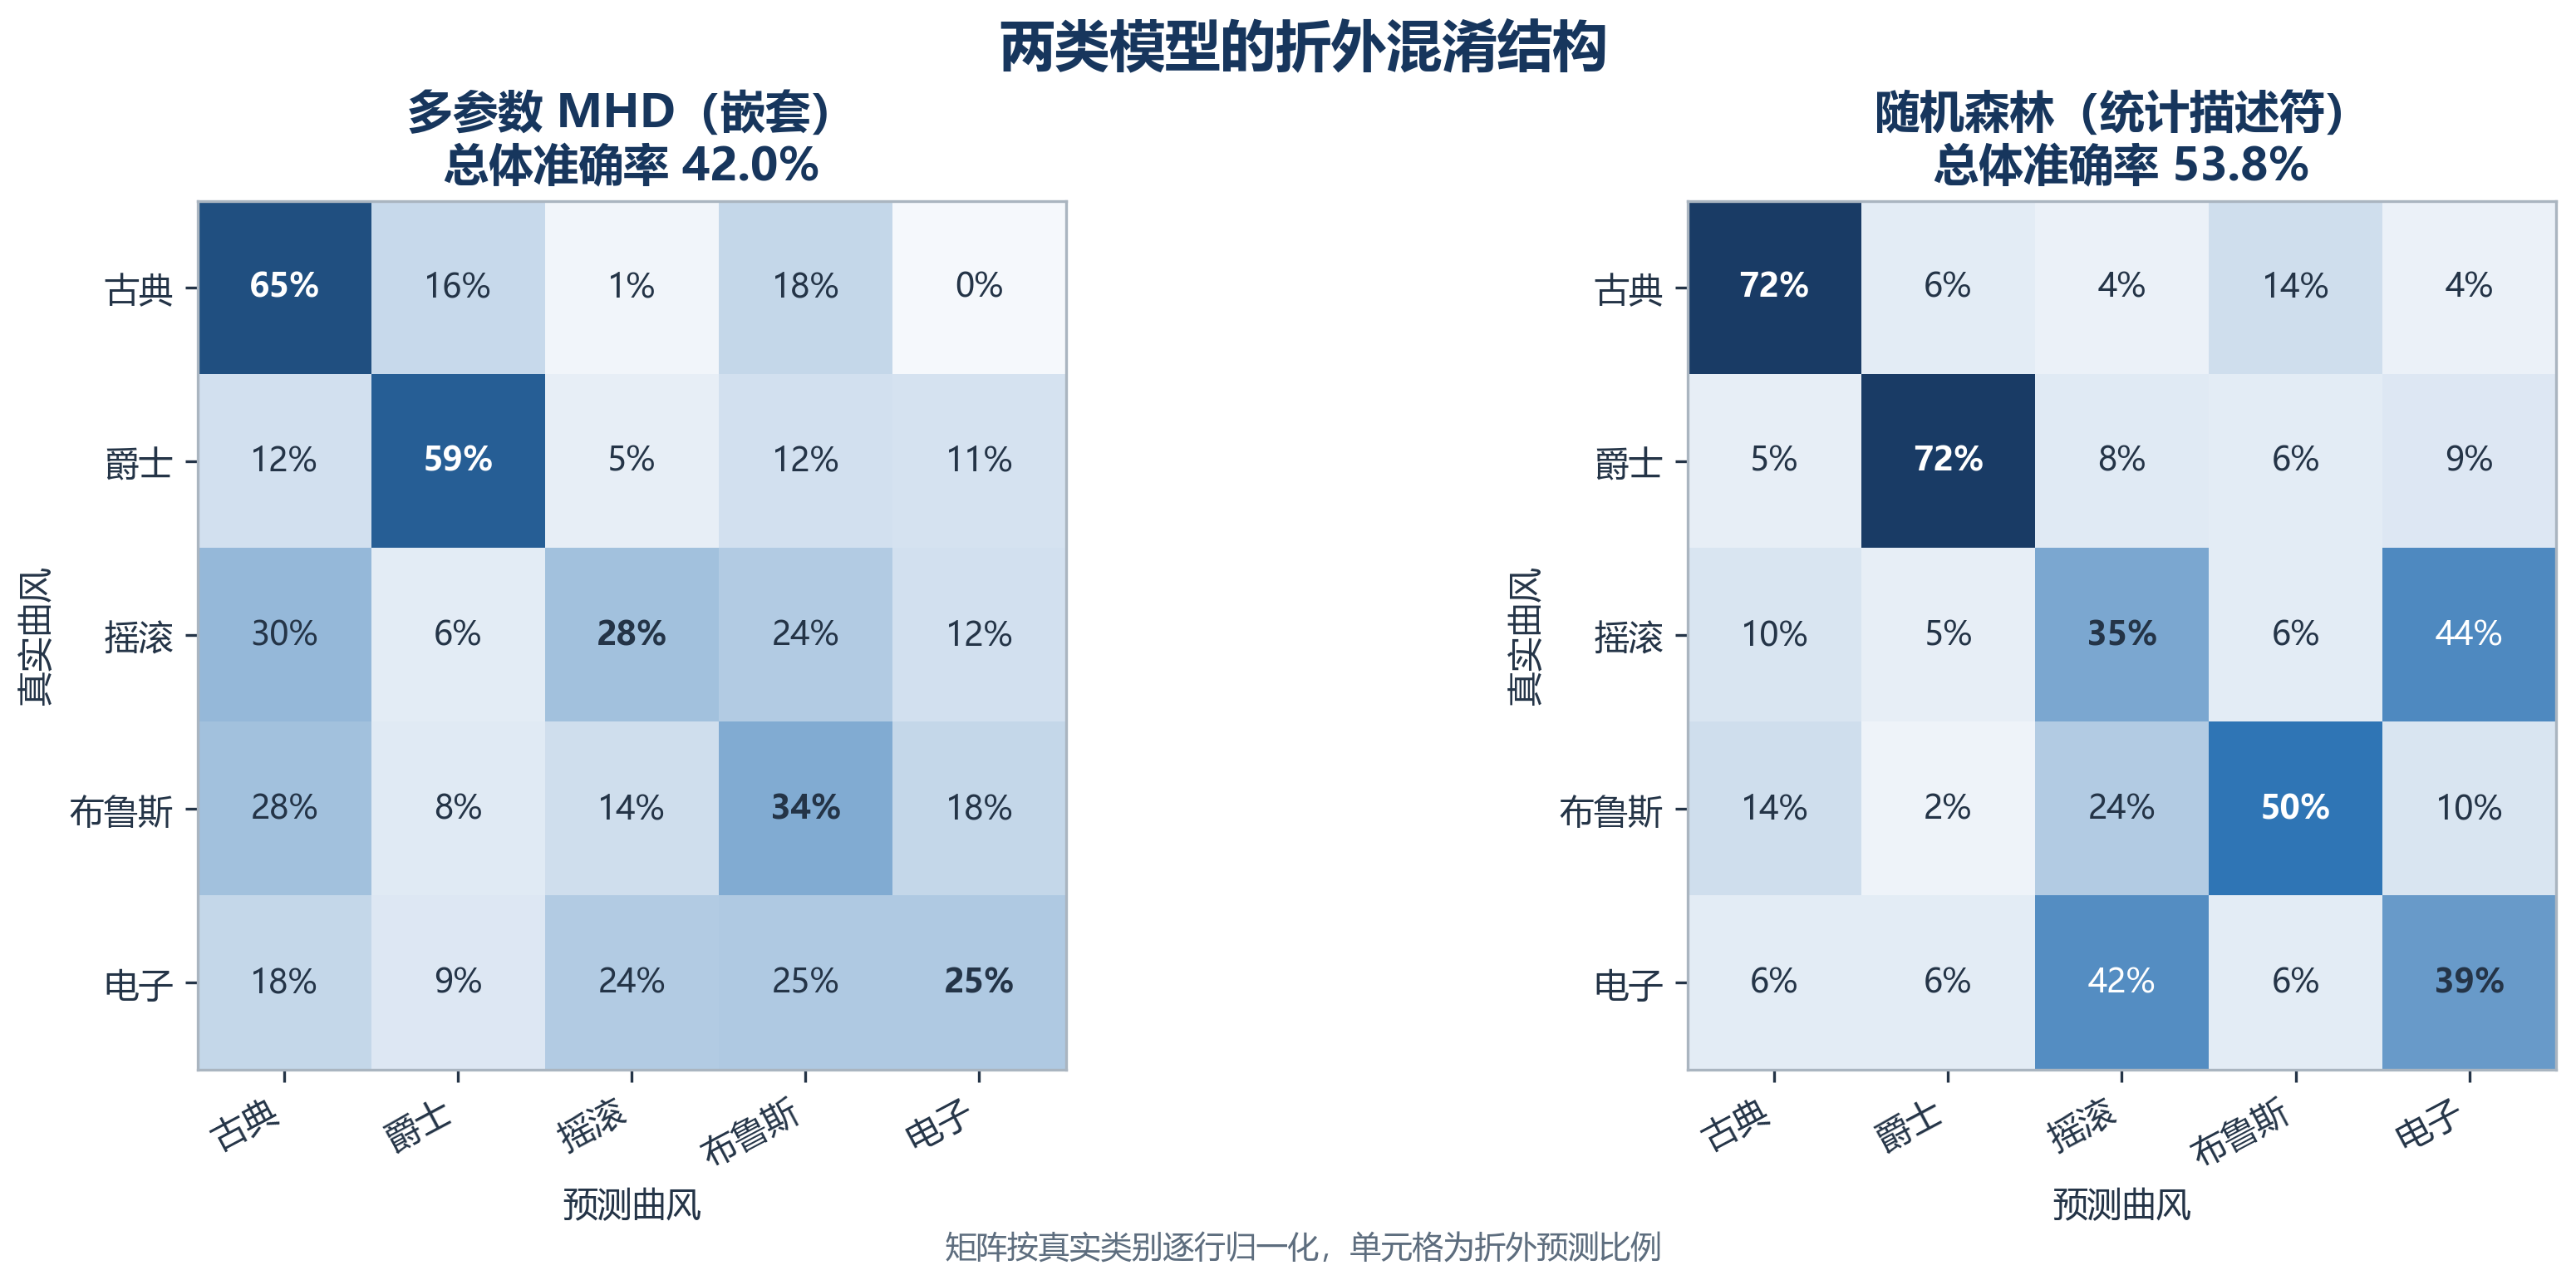
\includegraphics[width=0.98\textwidth]{confusion_models_cn.png}
  \caption{两类模型的归一化折外混淆矩阵}
  \label{fig:cmhd}
\end{figure}

图 \ref{fig:mds} 将固定权重 MHD 矩阵通过 MDS 映射到二维。各曲风存在局部聚集，
但分布椭圆总体仍大量重叠，与配对 AUC 仅 0.5759 的结果一致。该图提示
Hausdorff 空间具有弱簇结构，而非线性可分结构。

\begin{figure}[!htbp]
  \centering
  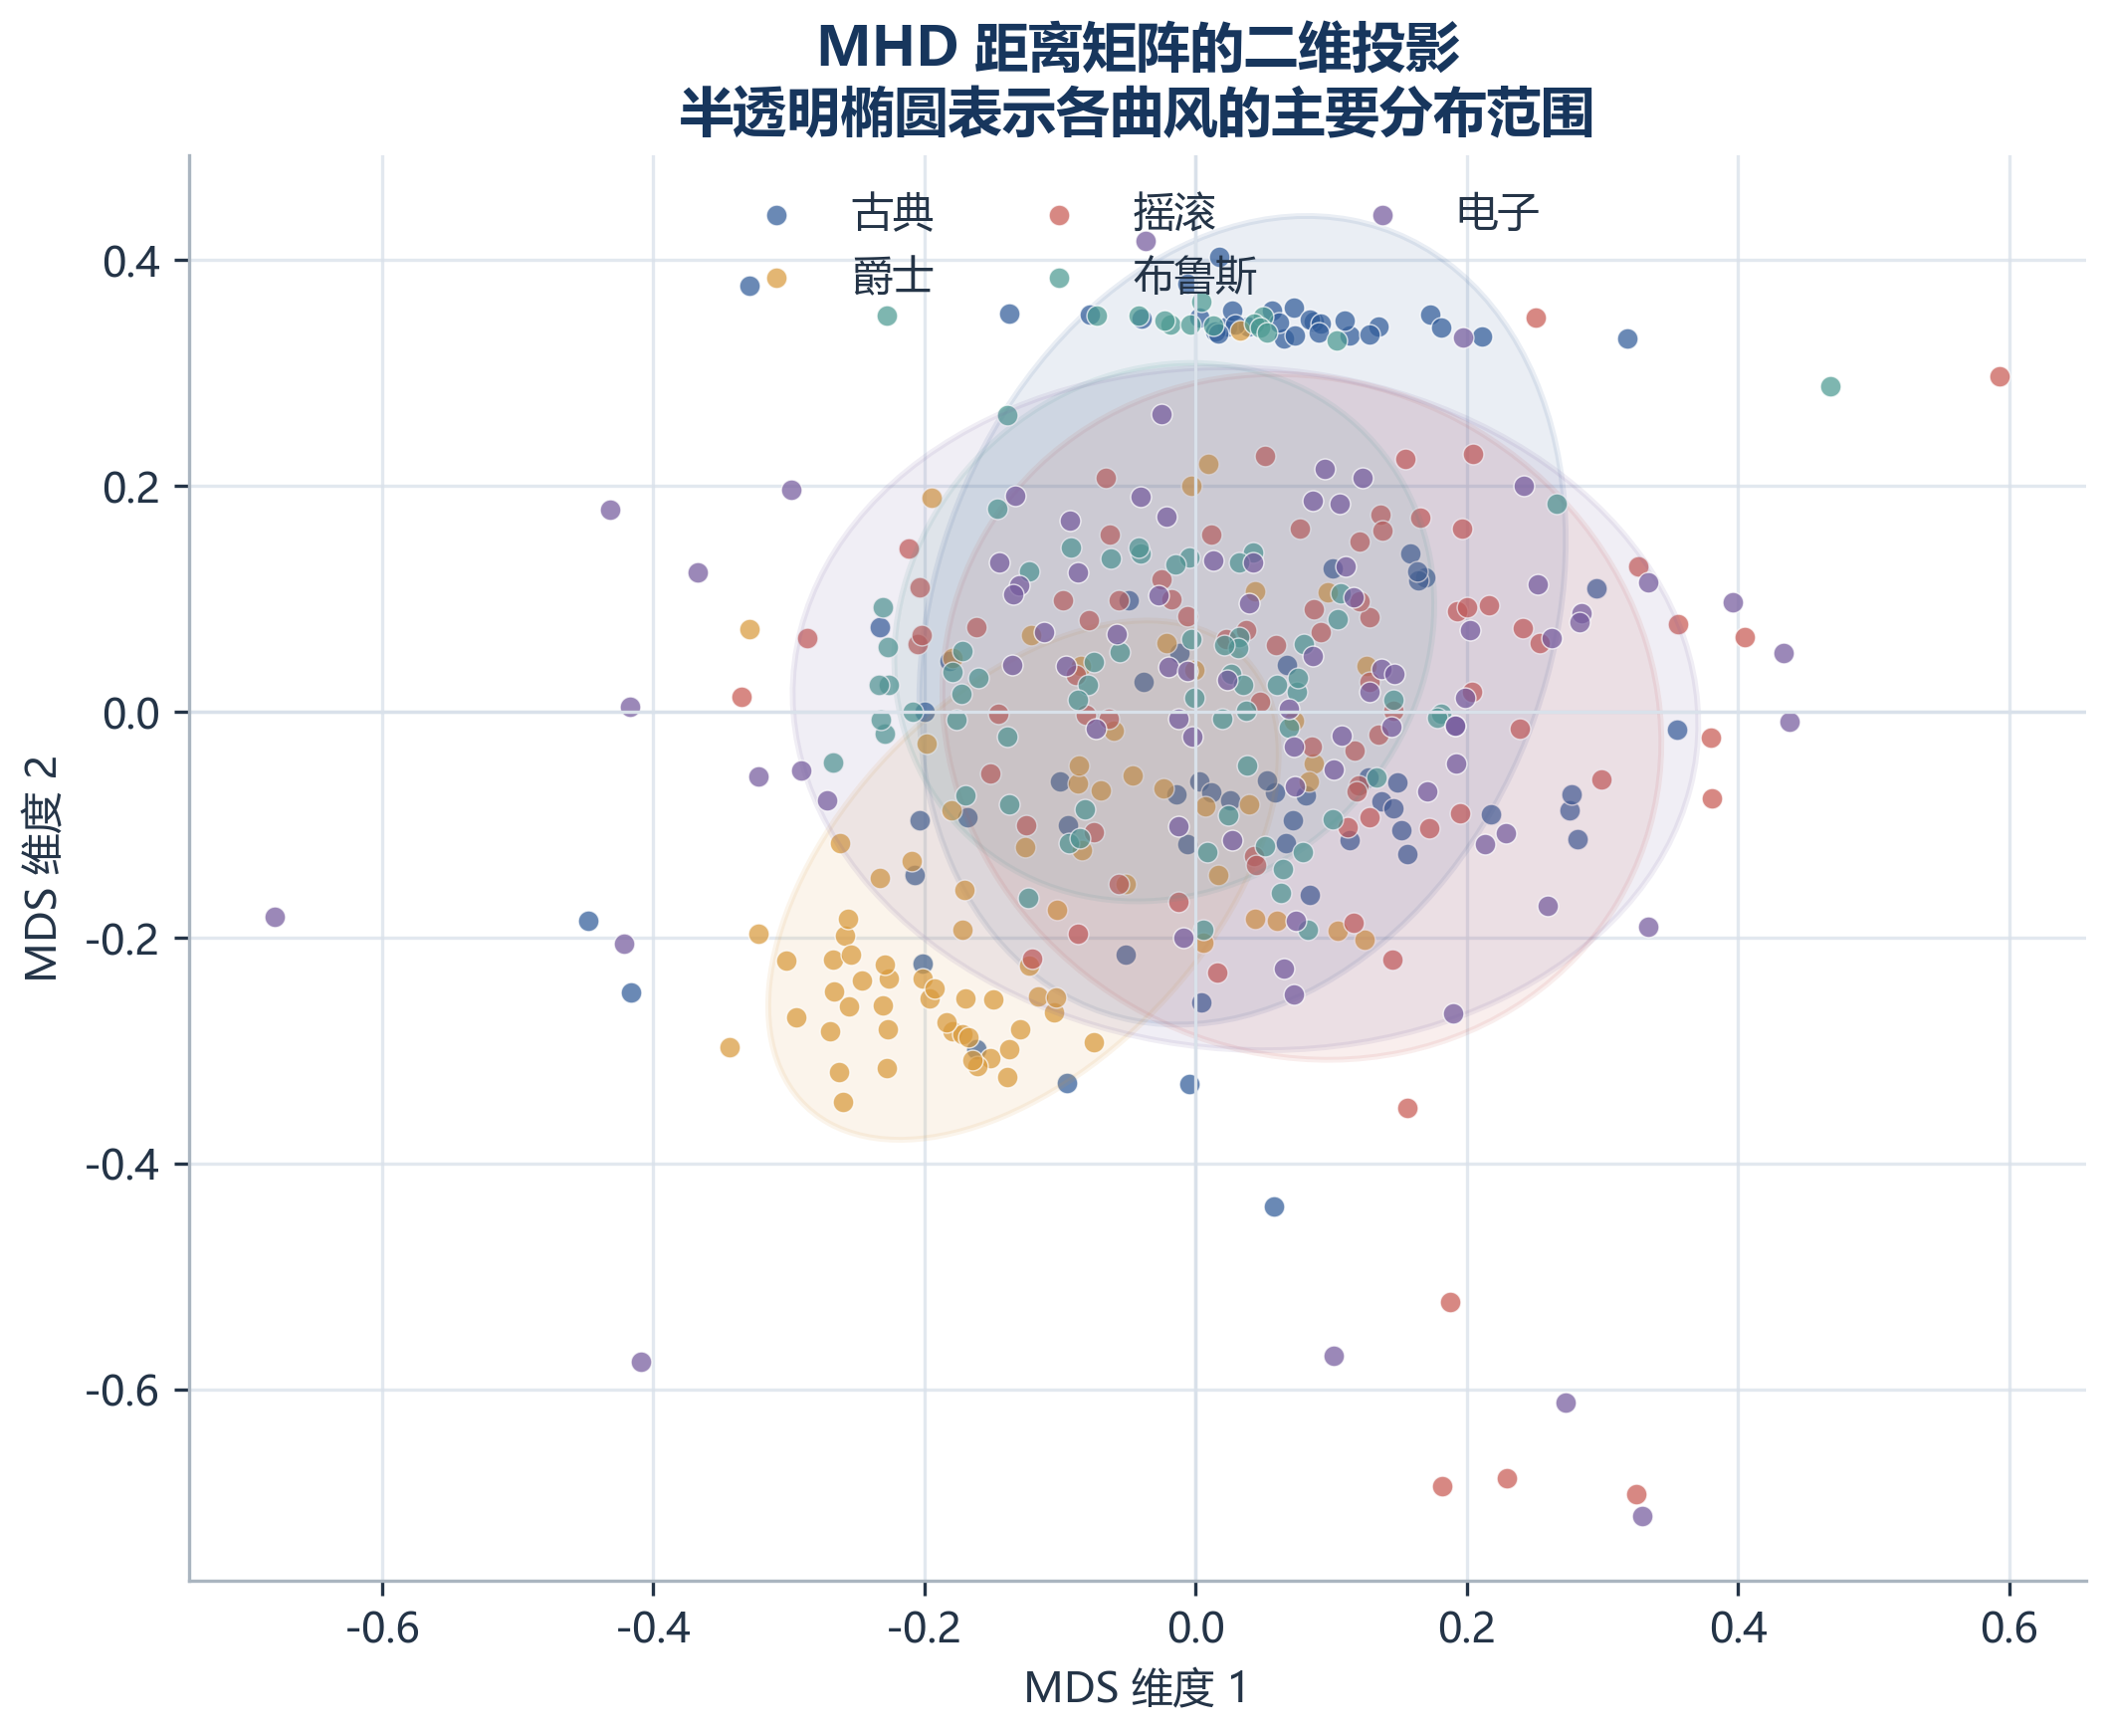
\includegraphics[width=0.78\textwidth]{mds_mhd_cn.png}
  \caption{MHD 距离矩阵的二维 MDS 投影}
  \label{fig:mds}
\end{figure}

\subsection{描述符模型解释}

随机森林采用每个外层测试折上的置换重要性，以“打乱某特征后平衡准确率的下降”
衡量贡献。排名前列的是音级熵、力度范围、起音间隔标准差、曲长、平均音高和
音高高分位数，见图 \ref{fig:importance}。这说明曲风不仅表现为三维轨迹的点集
形状，也表现为节奏不规则性、音级使用丰富度和力度动态等统计属性。单个重要性
数值较小还表明信息分散在多个相关描述符中，不宜把某一特征解释为唯一主因。

\begin{figure}[!htbp]
  \centering
  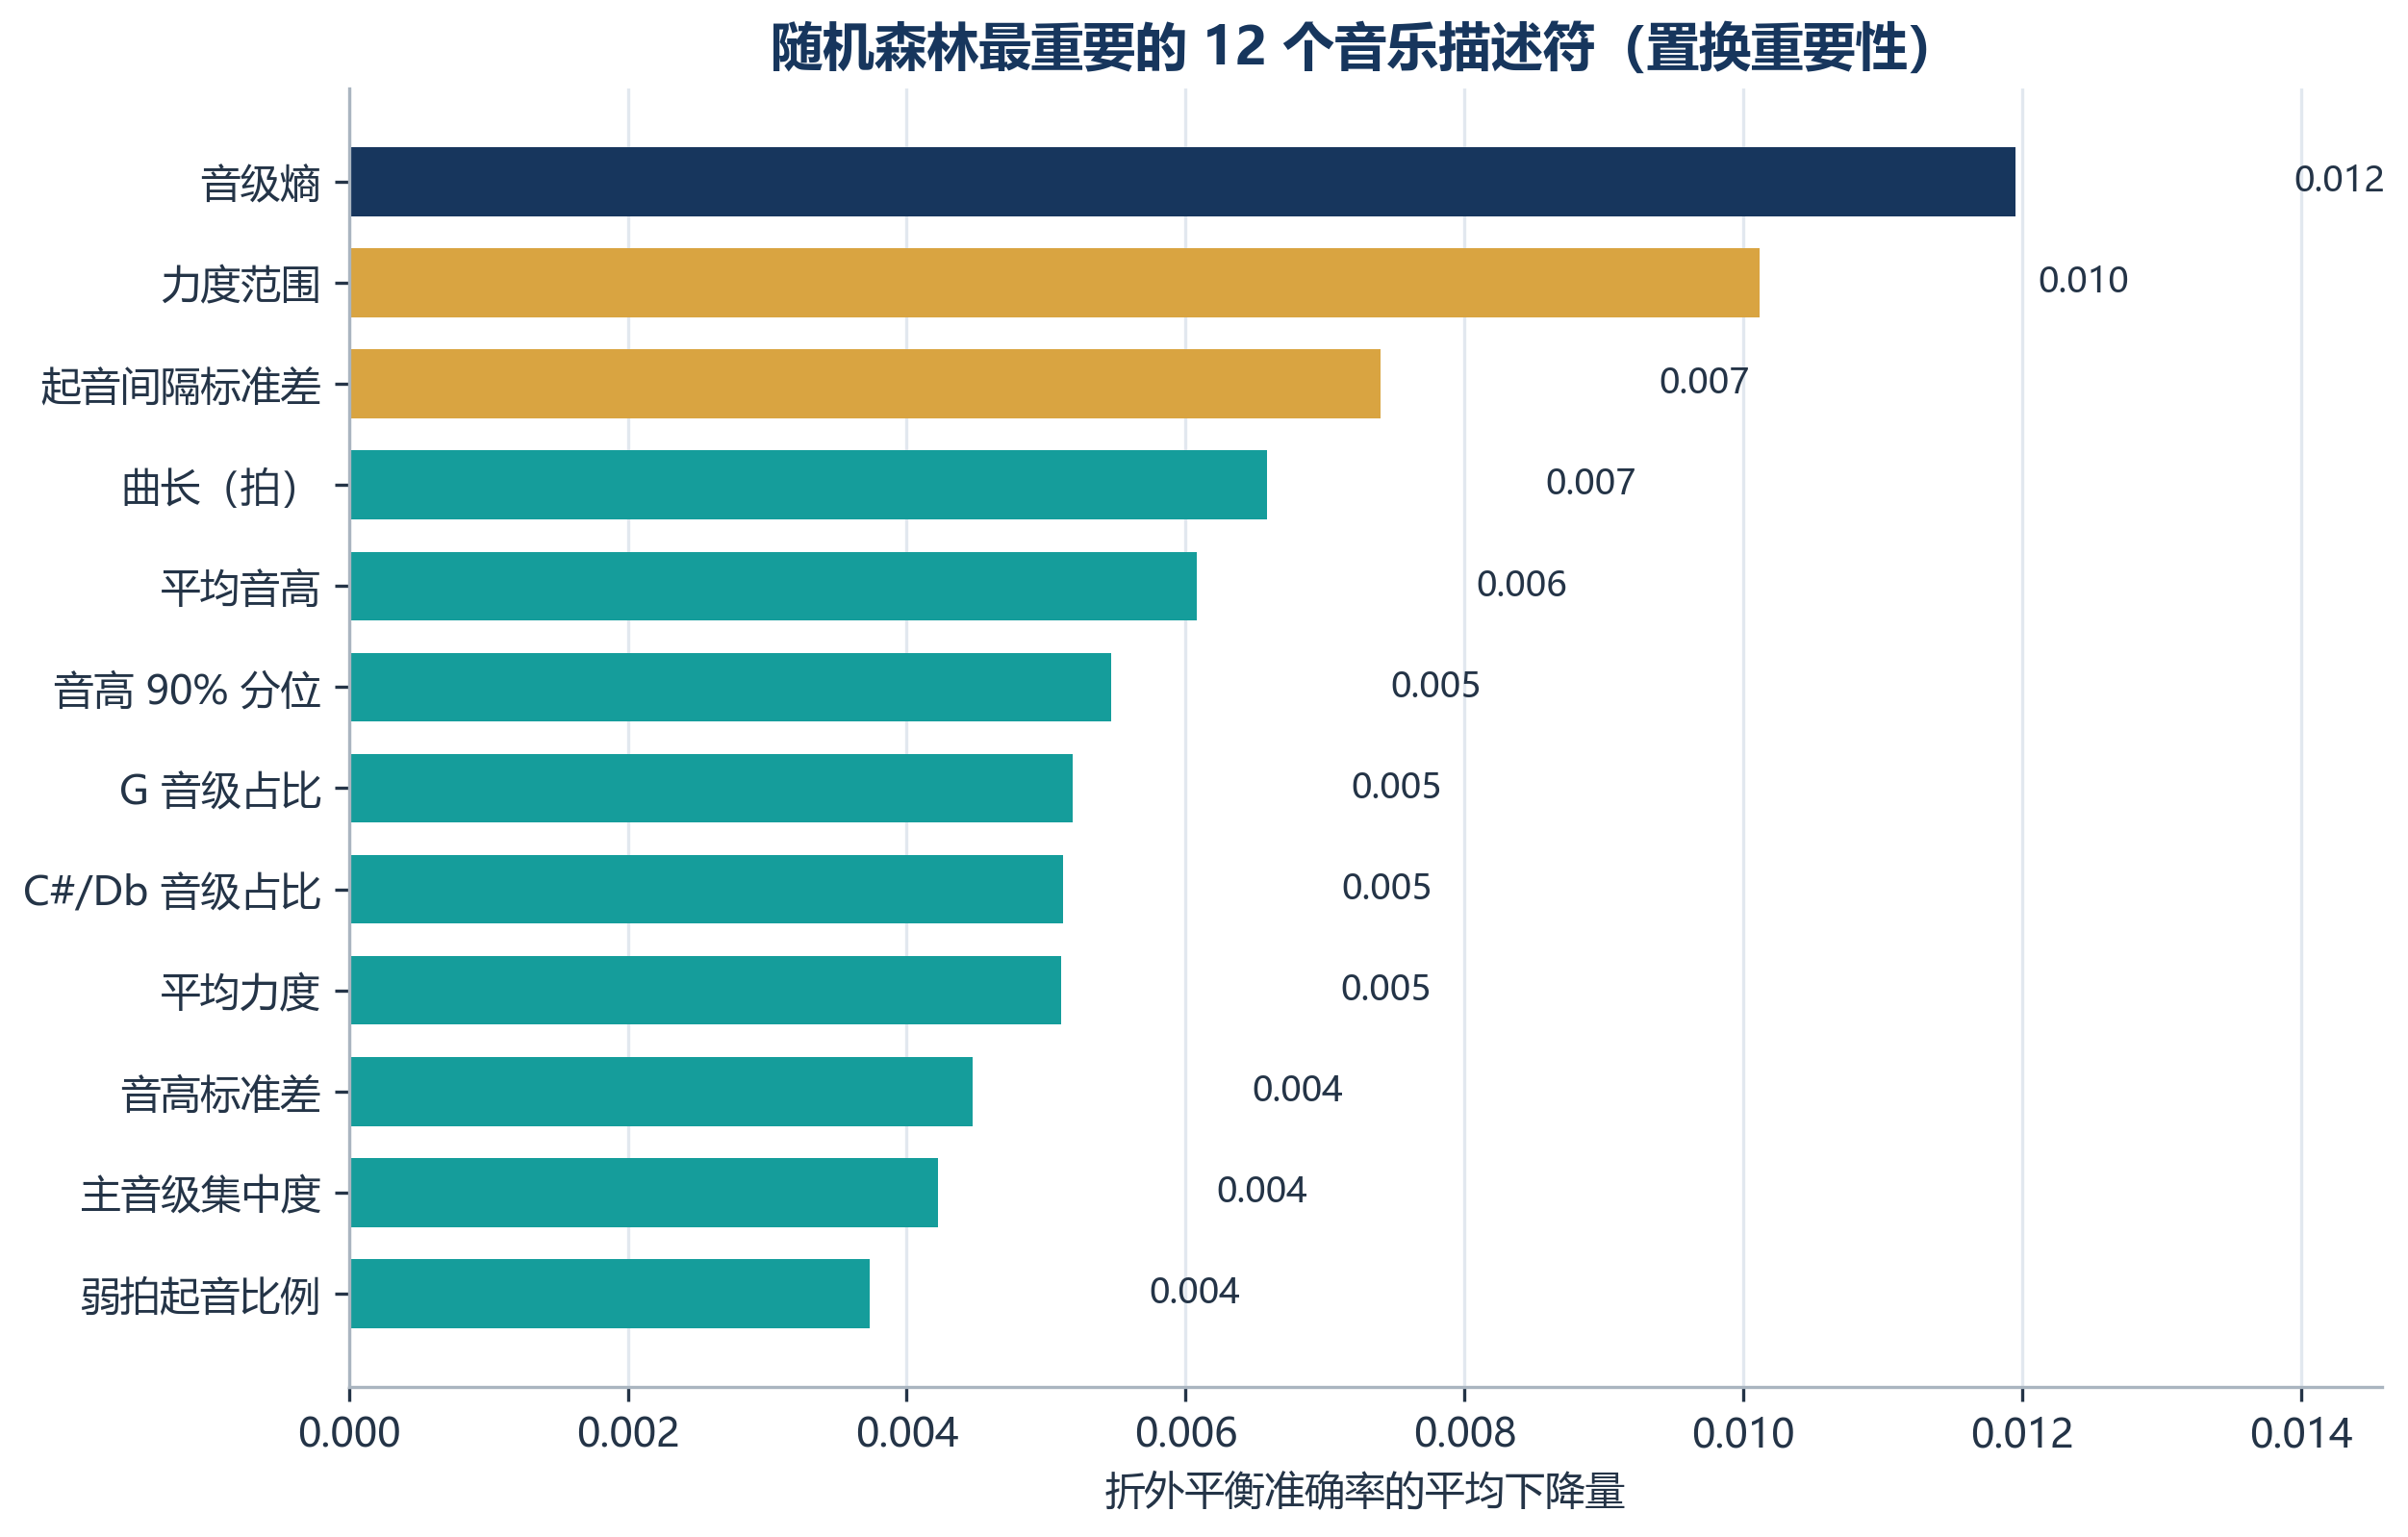
\includegraphics[width=0.76\textwidth]{feature_importance_cn.png}
  \caption{随机森林描述符的折外置换重要性}
  \label{fig:importance}
\end{figure}

\section{敏感性与稳健性分析}

\subsection{重采样点数}

把固定权重 MHD 曲线点数设为 48、72、96，准确率分别为 41.50\%、39.00\%
和 38.00\%。三者均高于随机基线，但性能并不随离散密度单调提高：48 点均值
最高，72 点折间波动最小。这说明过密采样可能放大局部装饰差异，不能先验认定
96 点最优，因此最终模型把点数纳入内层选择。

\subsection{音量权重}

固定权重实验中，$w_v=0,0.1,0.25,0.5$ 的准确率分别为 34.00\%、36.50\%、
38.00\%、40.00\%。音量维具有信息，但最优权重随数据折变化。正因如此，最终
模型不直接把 0.5 当作全局最优，而在每个外层训练折中重新选择权重。

\begin{figure}[!htbp]
  \centering
  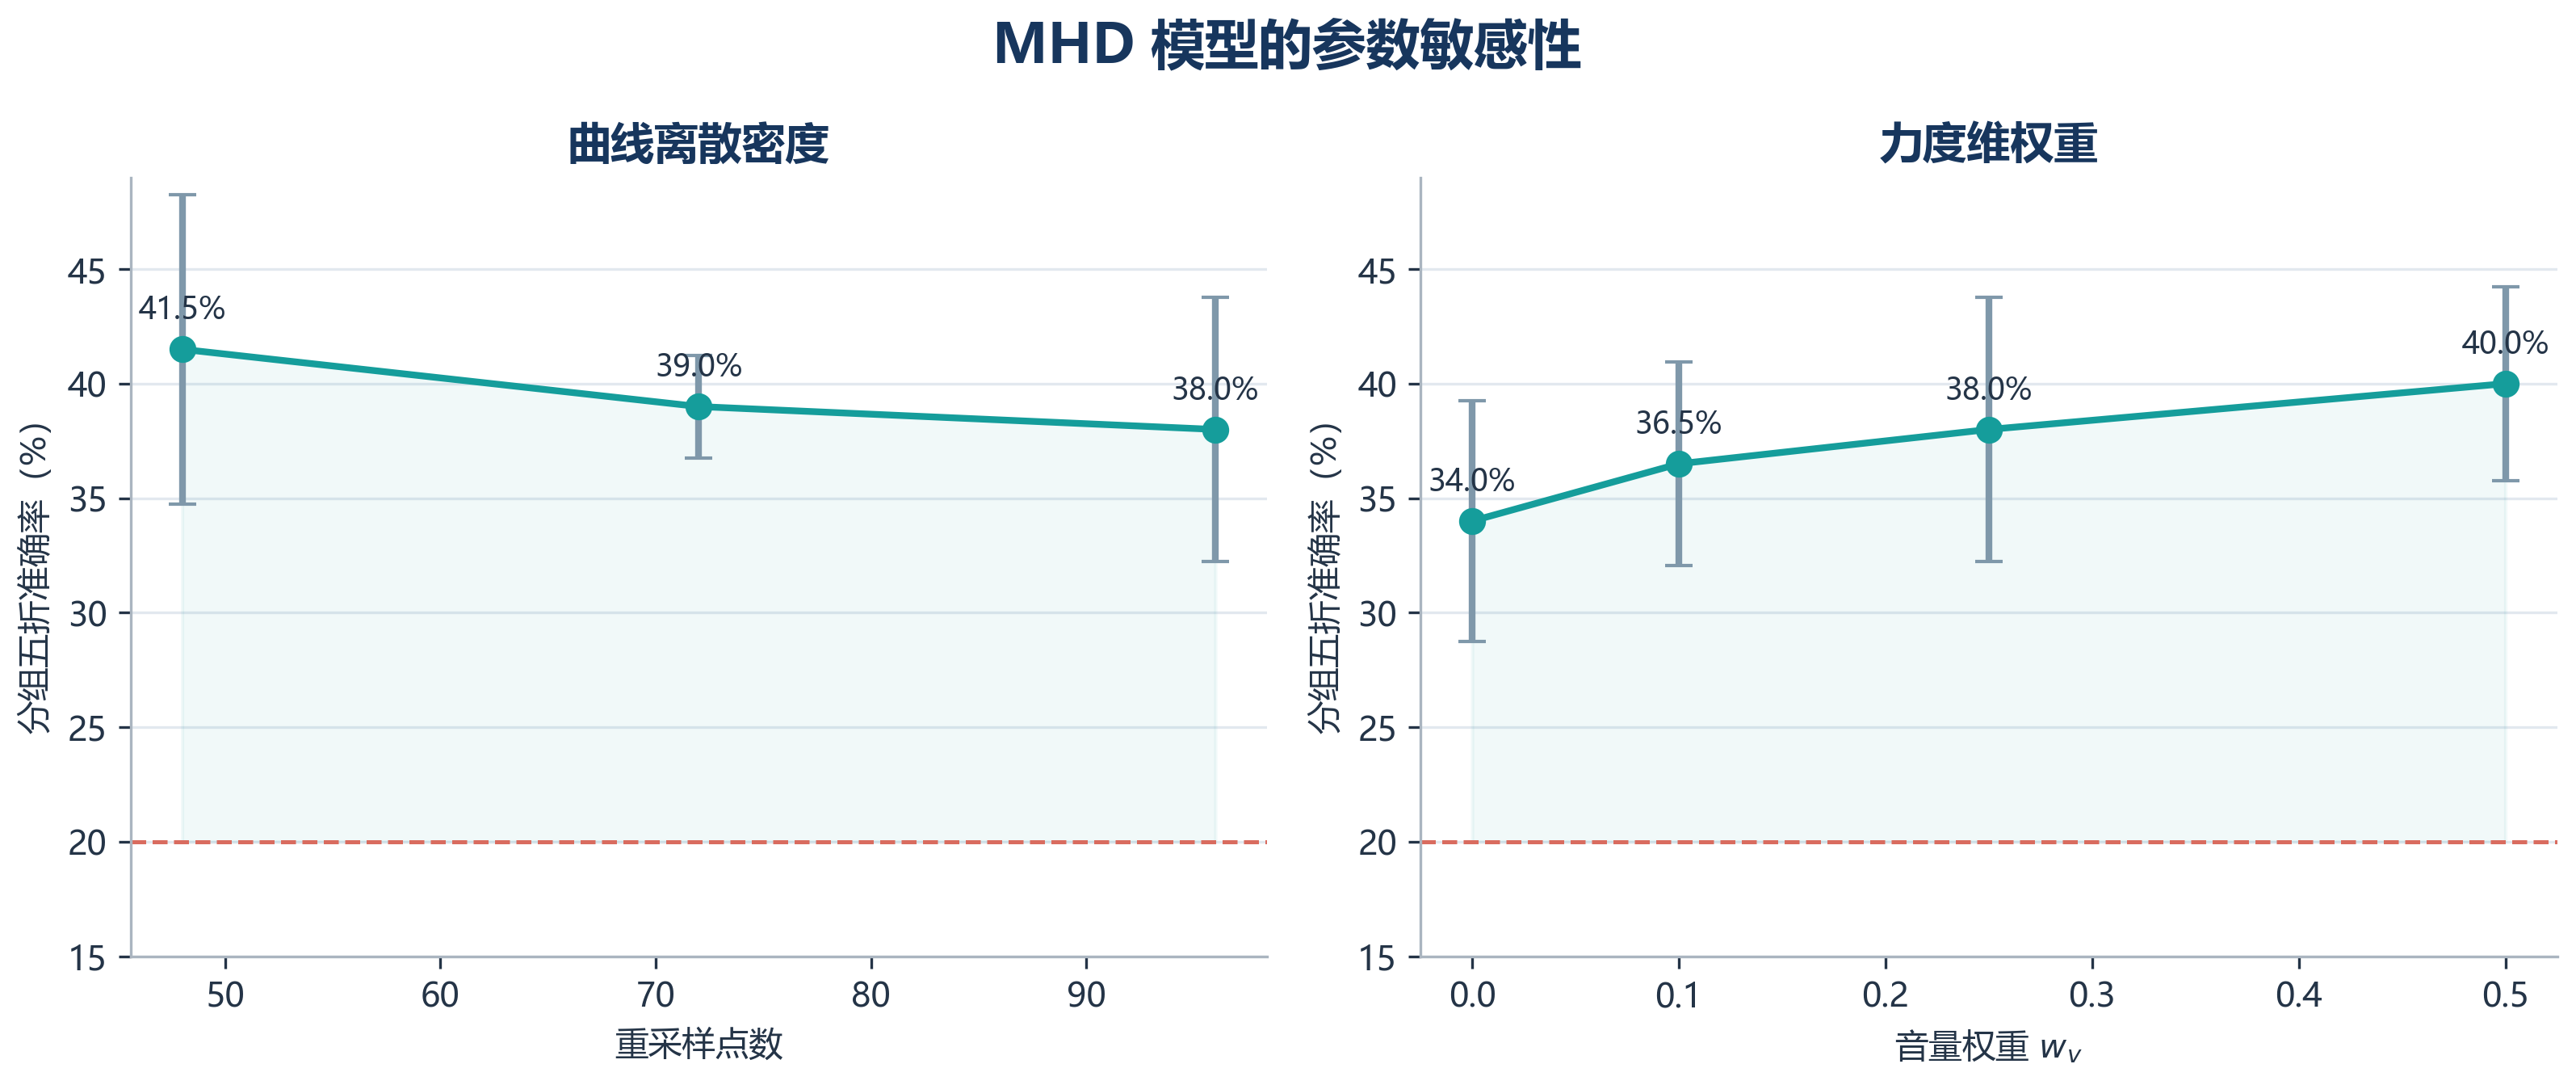
\includegraphics[width=0.92\textwidth]{sensitivity_cn.png}
  \caption{MHD 对重采样点数和音量权重的敏感性}
  \label{fig:sensitivity}
\end{figure}

\subsection{随机分折稳定性}

为检验结论是否依赖单一外层划分，本文使用随机种子 11、23、42、67、101
重复完整的分组五折流程。固定 MHD、多参数 MHD、随机森林的平均准确率分别为
$37.70\%\pm0.93\%$、$40.25\%\pm1.46\%$、$53.90\%\pm1.04\%$；多参数 MHD
的取值范围为 38.50\%--42.00\%。图 \ref{fig:repeat} 表明三类模型的排序在五组
划分中保持一致，主结论并非由某个“幸运分折”造成。

\begin{figure}[!htbp]
  \centering
  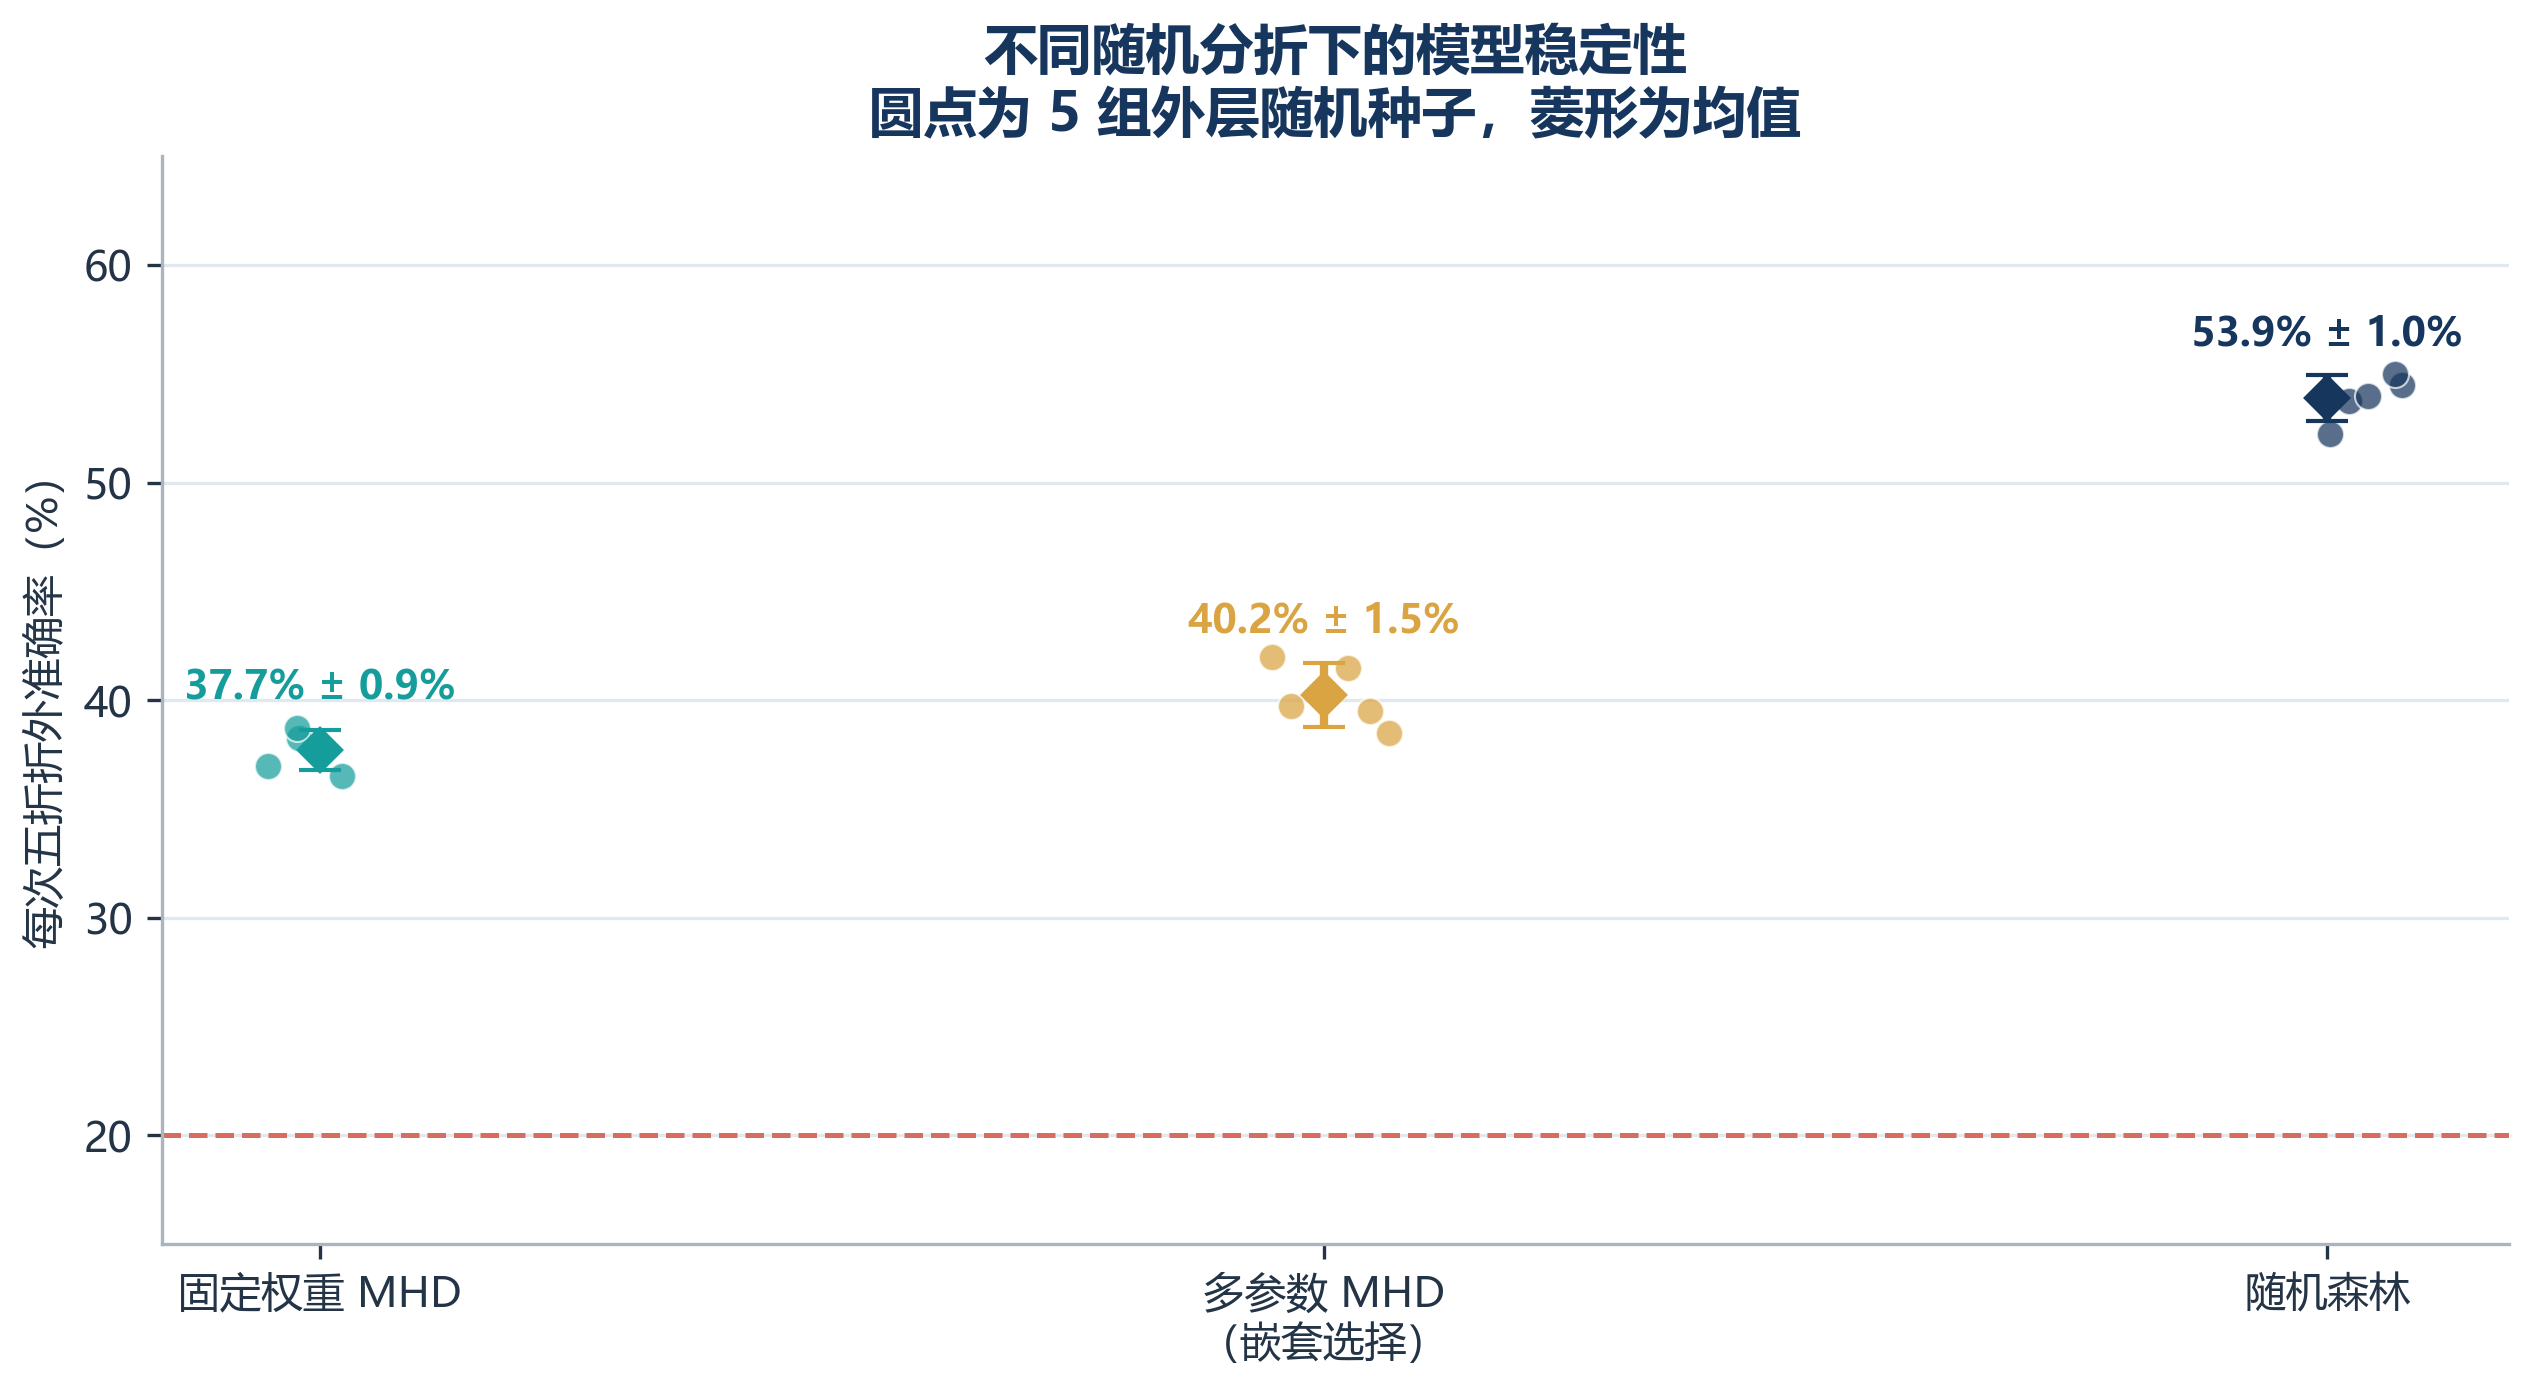
\includegraphics[width=0.80\textwidth]{repeated_validation_cn.png}
  \caption{五组外层随机分折下的模型稳定性}
  \label{fig:repeat}
\end{figure}

\section{模型评价}

\subsection{模型优点}

\begin{enumerate}[label=\arabic*.]
  \item \textbf{几何解释清晰。} 距离直接对应两条三维旋律线的最近点偏差，可
  解释为时间相位、相对音高和力度的综合差异。
  \item \textbf{验证设计严格。} 跨曲风同名作品先剔除，同曲不同版本在抽样前归组；
  每个曲名组只抽取一个版本，参数只在重复内层训练数据中选择，并额外检验五组
  外层随机划分，降低数据泄漏、测试集调参偏差和偶然分折影响。
  \item \textbf{改进有针对性。} Q95-HD 和 MHD 分别处理极端点敏感问题，加权
  表示处理三维重要性差异；每项改动均有合成或真实数据实验支持。
  \item \textbf{结论不过度外推。} 同类/异类差异虽显著，但 AUC 和分类精度表明
  效应有限，故将 Hausdorff 定位为有效基线和几何先验，而非完备分类器。
\end{enumerate}

\subsection{模型局限}

\begin{enumerate}[label=\arabic*.]
  \item 最高音 skyline 对复调作品只是近似，伴奏高音可能被误当作主旋律。
  \item Hausdorff 点集匹配不要求保持严格顺序，可能把走向相反但占据相似区域的
  旋律判为相似。
  \item ADL 的曲风标签由宽泛标签映射而来，Rock、Electronic 等大类内部差异大，
  标签噪声限制了可达到的精度。
  \item 数据仅保留钢琴声部，控制了音色变量，却也舍弃了真实曲风识别中极重要的
  配器和音色信息。
  \item 随机森林中的曲长可能同时反映数据来源和编曲习惯，不能全部解释为纯粹的
  音乐学规律。
\end{enumerate}

\subsection{可继续改进的方向}

后续可用动态规划或学习式声部跟踪替代最高音规则；将 Hausdorff 与离散
Fr\'echet、编辑距离、节奏直方图和调性特征融合；也可把旋律分成短乐句，先做
局部匹配再聚合，从而减少整曲归一化对局部主题的稀释。若面向实际曲风分类，
还应加入音色、和声与配器信息。

\section{结论}

本文建立了从 MIDI 音符到三维旋律曲线、从 Hausdorff 距离到曲风验证的完整
模型。400 首五类平衡数据上的结果表明：
\begin{enumerate}[label=\arabic*.]
  \item 同曲风旋律的 MHD 显著小于异曲风旋律，组级置换检验 $p=0.0005$，说明几何
  距离具有真实但较弱的曲风信息；
  \item 原始三维 Hausdorff 的分组五折准确率为 32.00\%，MHD 提升至 38.00\%，
  验证了降低离群点敏感性的必要性；
  \item 嵌套选择重采样点数、音量权重和近邻数后，多参数 MHD 达到
  $42.00\%\pm6.16\%$；五组外层随机划分的平均准确率为 40.25\%，约为随机
  基线的 2 倍；
  \item 多统计描述符随机森林达到 53.75\%，五次重复平均为 53.90\%，说明
  Hausdorff 最适合作为可解释的几何相似性组件，与节奏、音级和动态特征联合使用。
\end{enumerate}

因此，对题目所问“该度量在区分音乐曲风方面是否有效”，本文的回答是：
\textbf{有效，但有限。}它能够量化旋律线的几何接近程度并提供高于随机的曲风
区分能力，但不足以单独完成可靠的多曲风识别。

{\small
\begin{thebibliography}{99}
\setlength{\itemsep}{0.15em}

\bibitem{hausdorff}
Hausdorff F. \textit{Grundzüge der Mengenlehre}. Leipzig: Veit, 1914.

\bibitem{dubuisson}
Dubuisson M P, Jain A K. A modified Hausdorff distance for object matching[C].
Proceedings of the 12th International Conference on Pattern Recognition, 1994:
566--568.

\bibitem{dtw}
Sakoe H, Chiba S. Dynamic programming algorithm optimization for spoken word
recognition[J]. IEEE Transactions on Acoustics, Speech, and Signal Processing,
1978, 26(1): 43--49.

\bibitem{mir}
Müller M. \textit{Information Retrieval for Music and Motion}. Berlin:
Springer, 2007.

\bibitem{adl}
Ferreira L N, Lelis L H S, Whitehead J. Computer-generated music for tabletop
role-playing games[C]. Proceedings of the 16th AAAI Conference on Artificial
Intelligence and Interactive Digital Entertainment, 2020.

\bibitem{rf}
Breiman L. Random forests[J]. Machine Learning, 2001, 45: 5--32.

\end{thebibliography}
}

\appendix
\section{复现实验说明}

最终实验入口为项目根目录下的 \texttt{code/final\_experiment.py}。在本机
Anaconda 环境中执行：
\begin{lstlisting}[language=bash]
D:\app\Anaconda\python.exe code\final_experiment.py
D:\app\Anaconda\python.exe code\paper_assets.py
\end{lstlisting}

程序输出结构如下：
\begin{itemize}
  \item \texttt{results/final/cache/}：平衡抽样数据与距离矩阵缓存；
  \item \texttt{results/final/tables/}：机器可读的原始数值 CSV；
  \item \texttt{results/final/tables\_paper/}：带中文表头和统一精度的展示型 CSV；
  \item \texttt{results/final/figures\_paper/}：300 dpi 中文论文图件；
  \item \texttt{results/final/summary.json}：机器可读的完整结果摘要。
\end{itemize}
缓存文件名绑定流水线版本 \texttt{v2}，防止旧预处理结果被误复用；解析失败样本
及原因另存为 \texttt{sample\_failures.csv}。基础解析与距离性质由
\texttt{code/test\_pipeline.py} 中的回归测试复核，运行命令见 README。

\section{算法伪代码}

\begin{lstlisting}[
  language=Python,
  basicstyle=\ttfamily\footnotesize,
  caption={多参数 MHD 嵌套交叉验证}
]
for train, test in grouped_stratified_5fold:
    candidates = []
    for N, w, K in product([48, 72, 96],
                           [0, 0.1, 0.25, 0.5],
                           [1, 3, 5, 7, 9]):
        scores = [
            grouped_inner_3fold_score(D[N, w], K, train, seed)
            for seed in [2026, 2027, 2028]
        ]
        candidates.append((mean(scores), N, w, K))
    _, N_best, w_best, K_best = max(candidates)
    predict(test, D[N_best, w_best], K_best)
aggregate all out-of-fold predictions
\end{lstlisting}

\end{document}
